% ==============================================================================
% OVERLEAF COMPILATION INSTRUCTIONS:
% 1. Upload this entire folder structure to your Overleaf project.
% 2. Ensure the compiler is set to "pdfLaTeX" (default) or "XeLaTeX".
% 3. BibTeX/Biber engine is supported natively by Overleaf.
% 4. To use the official VIT emblem, upload "vit_logo.png" to the root directory
%    and uncomment the \includegraphics line in chapters/frontmatter.tex.
% ==============================================================================

\documentclass[12pt,a4paper,oneside]{report}

% === CORE TYPOGRAPHY & FONT ENCODING ===
\usepackage{mathptmx}           % Times New Roman text and math font
\usepackage[T1]{fontenc}
\usepackage[utf8]{inputenc}
\usepackage[a4paper, left=3.81cm, right=2.54cm, top=2.54cm, bottom=2.54cm]{geometry}
\usepackage{setspace}
\usepackage{fancyhdr}
\usepackage{graphicx}
\usepackage[dvipsnames,table]{xcolor}
\usepackage{array}
\usepackage{longtable}
\usepackage{booktabs}
\usepackage{tabularx}
\usepackage{multirow}
\usepackage{caption}
\usepackage{subcaption}
\usepackage{amsmath}
\usepackage{amssymb}
\usepackage{listings}
\usepackage{enumitem}
\usepackage{pdfpages}
\usepackage{titlesec}
\usepackage{tocloft}
\usepackage{tikz}
\usetikzlibrary{shapes.geometric, arrows, arrows.meta, positioning, fit, backgrounds, calc}

% === COLOR DEFINITIONS (ensures all diagram colors exist) ===
\definecolor{amber}{RGB}{255, 191, 0}
\definecolor{emerald}{RGB}{80, 200, 120}

% === TIKZ DIAGRAM HELPER COMMANDS ===
\providecommand{\pk}[1]{{\scriptsize\bfseries\color{blue!70!black}#1}}
\providecommand{\fk}[1]{{\scriptsize\color{gray!80!black}#1}}

% === TOC / LOF / LOT MARGIN ADJUSTMENTS (avoids overfull hbox in TOC) ===
\setlength{\cftsecnumwidth}{2.8em}
\setlength{\cftsubsecnumwidth}{3.6em}
\setlength{\cftsubsubsecnumwidth}{4.4em}
\setlength{\cftfignumwidth}{3.2em}
\setlength{\cfttabnumwidth}{3.2em}

% === FAST INLINE BIBLIOGRAPHY CONFIGURATION ===
\usepackage{cite}
\providecommand{\parencite}[1]{(\cite{#1})}
\providecommand{\textcite}[1]{\cite{#1}}

% === HYPERREF SETUP ===
\usepackage{hyperref}
\hypersetup{
  colorlinks=true,
  linkcolor=blue!70!black,
  citecolor=blue!70!black,
  urlcolor=cyan!70!black,
  pdftitle={Non Technical Skills Meeting Intelligence and Productivity Analysis System},
  pdfauthor={Yash Muthal, Mohd. Maaz Alam, Nikhil Kumar}
}

% === VIT CHENNAI FONT SIZE & FORMATTING SPECIFICATIONS ===
% Chapter heading: 16pt Bold Centered
\titleformat{\chapter}[display]
  {\normalfont\fontsize{16}{19}\bfseries\centering}
  {CHAPTER \thechapter}{0pt}{\vspace{-10pt}\fontsize{16}{19}\bfseries}
  [\vspace{6pt}]
\titlespacing*{\chapter}{0pt}{-25pt}{20pt}

% Section heading: 14pt Bold
\titleformat{\section}
  {\normalfont\fontsize{14}{17}\bfseries}
  {\thesection}{1em}{}
\titlespacing*{\section}{0pt}{14pt}{8pt}

% Subsection heading: 12pt Bold
\titleformat{\subsection}
  {\normalfont\fontsize{12}{15}\bfseries}
  {\thesubsection}{1em}{}
\titlespacing*{\subsection}{0pt}{10pt}{4pt}

% Subsubsection: 12pt Bold Italic
\titleformat{\subsubsection}
  {\normalfont\fontsize{12}{15}\bfseries\itshape}
  {\thesubsubsection}{1em}{}
\titlespacing*{\subsubsection}{0pt}{8pt}{3pt}

% === LINE SPACING ===
\onehalfspacing

% === PAGE NUMBERING ===
\pagestyle{fancy}
\fancyhf{}
\fancyfoot[C]{\thepage}
\renewcommand{\headrulewidth}{0pt}

% === PARAGRAPH SPECIFICATIONS ===
\setlength{\parindent}{0pt}
\setlength{\parskip}{8pt}

% === CODE LISTINGS FORMATTING ===
\lstset{
  basicstyle=\small\ttfamily,
  breaklines=true,
  frame=single,
  backgroundcolor=\color{gray!8},
  keywordstyle=\color{blue!70!black}\bfseries,
  commentstyle=\color{green!50!black}\itshape,
  stringstyle=\color{red!60!black},
  numbers=left,
  numberstyle=\tiny\color{gray},
  numbersep=8pt,
  captionpos=b,
  showspaces=false,
  showstringspaces=false
}

% Define JSON language for listings
\lstdefinelanguage{json}{
  basicstyle=\small\ttfamily,
  numbers=left,
  numberstyle=\tiny\color{gray},
  stepnumber=1,
  numbersep=8pt,
  showstringspaces=false,
  breaklines=true,
  frame=single,
  backgroundcolor=\color{gray!8},
  string=[s]{"}{"},
  stringstyle=\color{blue!80!black},
  comment=[l]{:},
  commentstyle=\color{black},
  morekeywords={true,false,null}
}

% === PROFESSIONAL FIGURE PLACEHOLDER MACRO ===
\newcommand{\figplaceholder}[3][12cm]{%
  \begin{figure}[htbp]
    \centering
    \resizebox{\linewidth}{!}{%
    \begin{tikzpicture}
      \draw[fill=gray!8, draw=gray!40, thick, rounded corners=5pt]
        (0,0) rectangle (12,4.5);
      \node[align=center] at (6,2.8) {\Large\color{gray!70}\textbf{[Figure Placeholder]}};
      \node[align=center, text width=10.5cm] at (6,1.6) {\normalsize\color{gray!60}\textit{#3}};
    \end{tikzpicture}%
    }
    \caption{#2}
    \label{fig:#2}
  \end{figure}
}

% === BEGIN DOCUMENT ===
\begin{document}

% Roman numeral numbering for Frontmatter
\pagenumbering{roman}
% ==============================================================================
% FRONTMATTER: Cover, Title, Declaration, Certificate, Abstract, Ack, TOC, Lists
% ==============================================================================

% ------------------------------------------------------------------------------
% 1. COVER PAGE
% ------------------------------------------------------------------------------
\begin{titlepage}
\thispagestyle{empty}
\begin{center}
  \vspace*{0.5cm}

  % Logo placeholder (Replace with \includegraphics[width=3.5cm]{vit_logo.png})
  
\begin{tikzpicture}
    \draw[thick, draw=blue!80!black, fill=blue!3, rounded corners=2pt] (0,0) rectangle (3.2, 3.2);
    \node at (1.6, 1.8) {\bfseries\small VIT LOGO};
    \node at (1.6, 1.1) {\tiny (Upload vit\_logo.png};
    \node at (1.6, 0.7) {\tiny to Overleaf root)};
  \end{tikzpicture}
  
  \vspace{0.8cm}
  
  {\fontsize{20}{24}\bfseries NON TECHNICAL SKILLS MEETING INTELLIGENCE AND PRODUCTIVITY ANALYSIS SYSTEM\par}
  
  \vspace{0.8cm}
  
  {\fontsize{13}{16}\itshape A Project Report Submitted in partial fulfillment of the requirements\\for the award of the degree of\par}
  
  \vspace{0.6cm}
  
  {\fontsize{16}{20}\bfseries BACHELOR OF TECHNOLOGY\\IN\\COMPUTER SCIENCE AND ENGINEERING\par}
  
  \vspace{0.8cm}
  
  {\fontsize{13}{16}\itshape by\par}
  
  \vspace{0.4cm}
  
  {\fontsize{14}{18}\bfseries
  YASH MUTHAL \quad (23BCE5002)\\[4pt]
  MOHD. MAAZ ALAM \quad (23BAI1426)\\[4pt]
  NIKHIL KUMAR \quad (23BAI1264)\par}
  
  \vfill
  
  {\fontsize{15}{18}\bfseries SCHOOL OF COMPUTER SCIENCE AND ENGINEERING\par}
  \vspace{0.2cm}
  {\fontsize{15}{18}\bfseries VELLORE INSTITUTE OF TECHNOLOGY, CHENNAI\par}
  \vspace{0.4cm}
  {\fontsize{12}{15}\bfseries NOVEMBER, 2025\par}

\end{center}
\end{titlepage}

% ------------------------------------------------------------------------------
% 2. TITLE PAGE (Identical format per VIT standard)
% ------------------------------------------------------------------------------
\begin{titlepage}
\thispagestyle{empty}
\begin{center}
  \vspace*{0.5cm}

  
\begin{tikzpicture}
    \draw[thick, draw=blue!80!black, fill=blue!3, rounded corners=2pt] (0,0) rectangle (3.2, 3.2);
    \node at (1.6, 1.8) {\bfseries\small VIT LOGO};
    \node at (1.6, 1.1) {\tiny (Upload vit\_logo.png};
    \node at (1.6, 0.7) {\tiny to Overleaf root)};
  \end{tikzpicture}
  
  \vspace{0.8cm}
  
  {\fontsize{20}{24}\bfseries NON TECHNICAL SKILLS MEETING INTELLIGENCE AND PRODUCTIVITY ANALYSIS SYSTEM\par}
  
  \vspace{0.8cm}
  
  {\fontsize{13}{16}\itshape A Project Report Submitted in partial fulfillment of the requirements\\for the award of the degree of\par}
  
  \vspace{0.6cm}
  
  {\fontsize{16}{20}\bfseries BACHELOR OF TECHNOLOGY\\IN\\COMPUTER SCIENCE AND ENGINEERING\par}
  
  \vspace{0.8cm}
  
  {\fontsize{13}{16}\itshape by\par}
  
  \vspace{0.4cm}
  
  {\fontsize{14}{18}\bfseries
  YASH MUTHAL \quad (23BCE5002)\\[4pt]
  MOHD. MAAZ ALAM \quad (23BAI1426)\\[4pt]
  NIKHIL KUMAR \quad (23BAI1264)\par}
  
  \vfill
  
  {\fontsize{15}{18}\bfseries SCHOOL OF COMPUTER SCIENCE AND ENGINEERING\par}
  \vspace{0.2cm}
  {\fontsize{15}{18}\bfseries VELLORE INSTITUTE OF TECHNOLOGY, CHENNAI\par}
  \vspace{0.4cm}
  {\fontsize{12}{15}\bfseries NOVEMBER, 2025\par}

\end{center}
\end{titlepage}

% ------------------------------------------------------------------------------
% 3. DECLARATION PAGE
% ------------------------------------------------------------------------------
\clearpage
\thispagestyle{plain}
\begin{center}
  {\fontsize{14}{17}\bfseries\underline{DECLARATION}\par}
\end{center}

\vspace{1.2cm}

I hereby declare that the project report entitled \textbf{"NON TECHNICAL SKILLS MEETING INTELLIGENCE AND PRODUCTIVITY ANALYSIS SYSTEM"} submitted by me to the School of Computer Science and Engineering, Vellore Institute of Technology, Chennai, in partial fulfillment of the requirements for the award of the degree of \textbf{Bachelor of Technology in Computer Science and Engineering}, is a bonafide record of original work carried out by me under the guidance and supervision of \textbf{Dr. Dhanush R}, Assistant Professor, School of Computer Science and Engineering, VIT Chennai.

I further declare that this report has not been submitted previously, in part or in full, to this or any other university or institution for the award of any degree, diploma, or other academic distinction.

\vspace{2.5cm}

\noindent
\begin{tabular*}{\textwidth}{@{\extracolsep{\fill}}lr}
\textbf{Place:} Chennai & \textbf{Signature of the Candidate} \\[0.4cm]
\textbf{Date:} \today   & \textbf{YASH MUTHAL} \\
                        & (Reg. No.: 23BCE5002)
\end{tabular*}

% ------------------------------------------------------------------------------
% 4. CERTIFICATE PAGE
% ------------------------------------------------------------------------------
\clearpage
\thispagestyle{plain}
\begin{center}
  {\fontsize{14}{17}\bfseries\underline{CERTIFICATE}\par}
\end{center}

\vspace{1.0cm}

This is to certify that the project report entitled \textbf{"NON TECHNICAL SKILLS MEETING INTELLIGENCE AND PRODUCTIVITY ANALYSIS SYSTEM"}, submitted by \textbf{YASH MUTHAL (Reg. No.: 23BCE5002)} in partial fulfillment of the requirements for the award of the degree of \textbf{Bachelor of Technology in Computer Science and Engineering} to the School of Computer Science and Engineering, Vellore Institute of Technology, Chennai, is a record of bonafide research work carried out under my supervision and guidance.

To the best of my knowledge, the matter embodied in this report has not been submitted to any other university or institute for the award of any degree or diploma.

\vspace{2.2cm}

\noindent
\begin{tabular*}{\textwidth}{@{\extracolsep{\fill}}p{6.8cm}p{6.8cm}@{}}
\textbf{Dr. Dhanush R} & \textbf{Dr. Prassanna J} \\
Project Guide & Professor \& Head of the Department \\
Assistant Professor, SCSE & School of Computer Science and Engineering \\
Vellore Institute of Technology, Chennai & Vellore Institute of Technology, Chennai
\end{tabular*}

\vspace{2.5cm}

\noindent
The candidate was evaluated in the viva-voce examination held on \rule{4cm}{0.4pt}.

\vspace{1.5cm}

\noindent
\begin{tabular*}{\textwidth}{@{\extracolsep{\fill}}p{6.8cm}p{6.8cm}@{}}
\textbf{Internal Examiner} & \textbf{External Examiner}
\end{tabular*}

% ------------------------------------------------------------------------------
% 5. ABSTRACT
% ------------------------------------------------------------------------------
\clearpage
\thispagestyle{plain}
\begin{center}
  {\fontsize{14}{17}\bfseries\MakeUppercase{Abstract}\par}
\end{center}
\vspace{0.6cm}

Modern organizational productivity critically depends on collaborative decision-making executed within physical and virtual meeting environments. While traditional meeting intelligence platforms focus predominantly on speech-to-text transcription and high-level lexical summaries, they overlook non-technical skills (NTS)---such as active listening, collaborative turn-taking, visual engagement, leadership assertion, and confidence---which constitute the true determinants of team efficacy. This project presents the \textbf{Non Technical Skills Meeting Intelligence and Productivity Analysis System (NTS-MIPA)}, an end-to-end, privacy-conscious multimodal behavioral intelligence platform designed to objectively quantify individual and team non-technical competencies during collaborative meetings.

The system incorporates an asynchronous, multi-tier decoupled microservice architecture featuring FastAPI, Node.js, Redis, and PostgreSQL with Row-Level Security (RLS). To capture intricate visual behavioral cues, a high-throughput computer vision pipeline is formulated utilizing \texttt{@vladmandic/human} and BlazeFace, extracting 468-point 3D facial landmark meshes, gaze deviation vectors, Perspective-n-Point (PnP) head pose kinematics (yaw, pitch, roll), and 7-class affective facial distributions sampled at 2 FPS. To eliminate identity swap anomalies common in conference tracking, an original \textit{Spatial X-Axis Anchor Tracking} algorithm is proposed, achieving deterministic, zero-swap identity persistence. For acoustic analysis, Faster-Whisper is deployed alongside a novel Mouth Aperture Ratio (MAR) visual-acoustic diarization fusion mechanism, resolving complex overlapping conversational turns. 

Features are temporally consolidated across 5-second sliding windows into a normalized 32-dimensional behavioral feature vector and evaluated via an optimized Random Forest Regressor ($N_{est}=150$), producing granular metric scores across five core NTS dimensions: Communication, Leadership, Engagement, Collaboration, and Confidence, in addition to behavioral archetype classification (Presenter, Facilitator, Collaborator, Observer). Furthermore, a physical CCTV room surveillance module powered by YOLOv8 and DeepSORT maps physical interaction zones via Picture-in-Picture (PIP) polygon projections. Evaluated across extensive benchmark recordings, NTS-MIPA achieves a processing Real-Time Factor (RTF) of $0.30\times$, a Diarization Error Rate (DER) of $8.1\%$, and an average Mean Absolute Error (MAE) of $0.051$ on NTS scoring ($R^2 = 0.894$). The solution delivers actionable personal coaching, interactive radar visualizations, and objective productivity analytics.

\vspace{0.8cm}
\noindent\textbf{Keywords:} Meeting Intelligence, Non-Technical Skills, Affective Computing, Facial Landmark Tracking, Visual-Acoustic Diarization, Faster-Whisper, Multimodal Fusion, Random Forest, CCTV Spatial Tracking.

% ------------------------------------------------------------------------------
% 6. ACKNOWLEDGEMENT
% ------------------------------------------------------------------------------
\clearpage
\thispagestyle{plain}
\begin{center}
  {\fontsize{14}{17}\bfseries\MakeUppercase{Acknowledgement}\par}
\end{center}
\vspace{0.6cm}

First and foremost, I express my profound gratitude to our Honorable Chancellor, \textbf{Dr. G. Viswanathan}, for providing world-class infrastructure and an intellectually stimulating environment at Vellore Institute of Technology, Chennai.

I express my deepest gratitude and sincere appreciation to my esteemed project guide, \textbf{Dr. Dhanush R}, Assistant Professor, School of Computer Science and Engineering, for his invaluable guidance, continuous encouragement, and insightful feedback throughout the conception and implementation of this project. His high standards of academic excellence and technical acumen served as a constant source of inspiration.

I extend my heartfelt thanks to \textbf{Dr. Prassanna J}, Professor and Head of the School of Computer Science and Engineering (SCSE), for providing the necessary institutional facilities, computing laboratories, and administrative support to carry out this research seamlessly.

I also extend my warmest appreciation to my dedicated project teammates, \textbf{Mohd. Maaz Alam} (23BAI1426) and \textbf{Nikhil Kumar} (23BAI1264), whose collaborative synergy, technical contributions in audio processing and physical tracking modules, and persistent camaraderie made the successful realization of this system possible.

Finally, I would like to convey my eternal indebtedness to my parents and family members for their constant prayers, moral support, and unconditional sacrifices that enabled me to pursue my academic aspirations.

\vspace{1.8cm}
\noindent
\begin{tabular*}{\textwidth}{@{\extracolsep{\fill}}lr}
\textbf{Place:} Chennai & \textbf{YASH MUTHAL} \\
\textbf{Date:} \today   & (Reg. No.: 23BCE5002)
\end{tabular*}

% ------------------------------------------------------------------------------
% 7. TABLE OF CONTENTS
% ------------------------------------------------------------------------------
\clearpage
\tableofcontents

% ------------------------------------------------------------------------------
% 8. LIST OF TABLES
% ------------------------------------------------------------------------------
\clearpage
\listoftables

% ------------------------------------------------------------------------------
% 9. LIST OF FIGURES
% ------------------------------------------------------------------------------
\clearpage
\listoffigures

% ------------------------------------------------------------------------------
% 10. LIST OF ABBREVIATIONS
% ------------------------------------------------------------------------------
\clearpage
\begin{center}
  {\fontsize{14}{17}\bfseries\MakeUppercase{List of Abbreviations}\par}
\end{center}
\vspace{0.6cm}

\begin{longtable}{@{}p{3.0cm}p{11.0cm}@{}}
\toprule
\textbf{Abbreviation} & \textbf{Full Expansion} \\
\midrule
\endfirsthead
\toprule
\textbf{Abbreviation} & \textbf{Full Expansion} \\
\midrule
\endhead
\bottomrule
\endfoot

\textbf{API}     & Application Programming Interface \\
\textbf{ARQ}     & Asynchronous Redis Queue \\
\textbf{ASR}     & Automatic Speech Recognition \\
\textbf{CCTV}    & Closed-Circuit Television \\
\textbf{CORS}    & Cross-Origin Resource Sharing \\
\textbf{CV}      & Computer Vision \\
\textbf{DER}     & Diarization Error Rate \\
\textbf{ER}      & Entity-Relationship \\
\textbf{FACS}    & Facial Action Coding System \\
\textbf{FFmpeg}  & Fast Forward Moving Picture Experts Group \\
\textbf{FPS}     & Frames Per Second \\
\textbf{GPU}     & Graphics Processing Unit \\
\textbf{HOD}     & Head of the Department \\
\textbf{HTML}    & HyperText Markup Language \\
\textbf{JSON}    & JavaScript Object Notation \\
\textbf{JSONB}   & Binary JavaScript Object Notation \\
\textbf{JWT}     & JSON Web Token \\
\textbf{MAE}     & Mean Absolute Error \\
\textbf{MAR}     & Mouth Aperture Ratio \\
\textbf{MIPA}    & Meeting Intelligence and Productivity Analysis \\
\textbf{ML}      & Machine Learning \\
\textbf{NFR}     & Non-Functional Requirement \\
\textbf{NTS}     & Non-Technical Skills \\
\textbf{PIP}     & Picture-in-Picture \\
\textbf{PnP}     & Perspective-n-Point \\
\textbf{RBAC}    & Role-Based Access Control \\
\textbf{REST}    & Representational State Transfer \\
\textbf{RLS}     & Row-Level Security \\
\textbf{RTF}     & Real-Time Factor \\
\textbf{SCSE}    & School of Computer Science and Engineering \\
\textbf{SORT}    & Simple Online and Realtime Tracking \\
\textbf{SPA}     & Single Page Application \\
\textbf{STT}     & Speech-to-Text \\
\textbf{TOC}     & Table of Contents \\
\textbf{UML}     & Unified Modeling Language \\
\textbf{VAD}     & Voice Activity Detection \\
\textbf{VIT}     & Vellore Institute of Technology \\
\textbf{WER}     & Word Error Rate \\
\textbf{WPM}     & Words Per Minute \\
\textbf{WSS}     & WebSocket Secure \\
\textbf{YOLO}    & You Only Look Once \\
\bottomrule
\end{longtable}


% Arabic numeral numbering from Chapter 1 onward
\clearpage
\pagenumbering{arabic}
\setcounter{page}{1}

\chapter{INTRODUCTION}

\section{BACKGROUND AND CONTEXT}
In contemporary knowledge-driven corporate and academic environments, meetings represent the primary vehicle for strategic alignment, collaborative problem-solving, intellectual consensus, and decision execution. Studies in organizational psychology indicate that mid-level and executive professionals allocate upwards of $35\%$ to $60\%$ of their working hours to participating in or facilitating group discussions, cross-functional sprints, and administrative committee meetings. While technical proficiency provides the fundamental competency necessary for task execution, modern organizational productivity is overwhelmingly dictated by what behavioral researchers term \textit{Non-Technical Skills} (NTS) \parencite{helmreich2004notechs, fletcher2003notss}. 

Non-technical skills encompass an individual's cognitive and interpersonal abilities that complement technical expertise to ensure safe, efficient, and cohesive group operations. Specifically, these skills manifest as active listening, verbal and non-verbal assertiveness, situational awareness, emotional regulation, collaborative turn-taking, and confidence exhibition. In high-stakes industries such as commercial aviation (where the NOTECHS framework originated) and surgical operations (evaluated via the NOTSS taxonomy), the quantitative appraisal of non-technical skills has long been recognized as a mandatory prerequisite for operational safety and human error mitigation \parencite{fletcher2003notss, vinciarelli2009social}. Conversely, within enterprise corporate boardrooms and higher-education research laboratories, the evaluation of human collaborative dynamics has historically remained subjective, anecdotal, and qualitative.

Traditional methodologies for assessing meeting effectiveness and participant interpersonal competency rely on manual human observation or retrospective self-report questionnaires. These legacy paradigms suffer from three debilitating systemic vulnerabilities:
\begin{enumerate}[label=(\roman*)]
    \item \textbf{Observer Cognitive Bias and Subjectivity:} Human observers inevitably evaluate participants through latent cognitive lenses, including recency bias, the halo effect, confirmation bias, and gender or cultural preconceptions, leading to inconsistent and uncalibrated performance reviews.
    \item \textbf{Temporal Infeasibility and Lack of Granularity:} A human rater cannot simultaneously monitor the micro-expressions, continuous gaze trajectories, vocal pitch inflections, and conversational transition gaps of multiple participants across an extended 60-minute conference. Consequently, subtle behavioral cues and micro-interactions are permanently lost.
    \item \textbf{Operational Cost and Non-Scalability:} Deploying trained industrial-organizational psychologists or professional behavioral coaches to audit routine enterprise interactions imposes prohibitive financial and logistical costs, restricting systematic performance coaching strictly to senior C-suite executives.
\end{enumerate}

The simultaneous maturation of artificial intelligence, high-throughput affective computing, deep learning computer vision frameworks, and transformer-based automatic speech recognition (ASR) has created an unprecedented paradigm shift \parencite{radford2023robust, baevski2020wav2vec}. Multimodal artificial intelligence now affords the capability to capture, synchronize, and interpret multi-sensory human behavioral signals at millisecond resolution. By processing facial geometry, eye gaze dynamics, acoustic prosody, conversational latency, and physical spatial presence concurrently, computational systems can construct objective, reproducible, and privacy-conscious behavioral profiles of collaborative interactions.

\section{EVOLUTION OF MEETING INTELLIGENCE SYSTEMS}
To position the architectural necessity of the proposed platform, it is imperative to analyze the historical evolution of computational meeting analysis over the preceding three decades. As delineated below, meeting intelligence technologies have transitioned across three distinct technological epochs.

\subsection{First Generation: Passive Recording and Archival Systems (1995--2010)}
The initial paradigm of digital meeting management focused exclusively on raw media acquisition, audio-visual encoding, and centralized file indexing. Technologies during this period centered around hardware room codecs (e.g., Polycom, Cisco Tandberg) that generated static audio-video recordings stored on local network-attached servers. In these systems, meetings remained unstructured, opaque multimedia blobs. To extract intelligence or review a critical discussion item, stakeholders were compelled to manually seek through hours of footage. No algorithmic understanding of conversation structure, participant contribution, or speaker identity existed.

\subsection{Second Generation: Text-Centric ASR and Lexical Analytics (2011--2022)}
The commercialization of cloud telephony and deep learning speech recognition ushered in the second generation of meeting intelligence, epitomized by cloud software offerings such as Otter.ai, Zoom Automatic Transcripts, Gong.io, and Microsoft Teams Transcription \parencite{gong2021revenue, blanco2020meeting}. These platforms harness acoustic acoustic-to-text models (such as Conformer or standard Whisper architectures) to convert spoken dialogue into searchable transcripts, subsequently feeding text streams into Large Language Models (LLMs) to generate post-meeting summaries, action items, and basic keyword sentiment.

Despite their ubiquity, second-generation platforms suffer from fundamental architectural blind spots:
\begin{itemize}
    \item \textbf{Visual Blindness:} Over $70\%$ of interpersonal human communication is communicated via non-verbal channels, including facial affect, nodding, eye contact, and head orientation \parencite{ekman1978facial, vinciarelli2009social}. Textual transcriptions completely discard these vital non-verbal signals.
    \item \textbf{Acoustic Diarization Degradation:} In physical conference rooms equipped with a single omnidirectional ceiling microphone or laptop array, standard acoustic speaker diarization suffers catastrophic failure during overlapping talk, cross-talk, and reverberant acoustic reflection, producing high Diarization Error Rates (DER) exceeding $25\%$.
    \item \textbf{Absence of Behavioral Quantification:} Current systems merely report \textit{what} was said, failing entirely to quantify \textit{how} individuals interact, whether listeners are actively engaged, or whether communication dynamics foster psychological safety.
\end{itemize}

\subsection{Third Generation: Multimodal Behavioral Intelligence (The Proposed System)}
The third generation of meeting intelligence represents a foundational leap from textual logging to holistic multimodal behavioral fusion. The \textbf{NTS-MIPA System} conceived in this project embodies this paradigm by fusing high-framerate 3D facial geometry, head pose kinematics, iris gaze stability, vocal prosodic dynamics, visual-assisted speaker diarization, and physical room tracking into a unified temporal analytical engine. Rather than relying solely on lexical transcriptions, third-generation systems continuously quantify non-technical competencies, diagnose systemic conversational imbalances, and generate actionable, bias-free behavioral development feedback.

\section{PROBLEM STATEMENT}
Meeting analytics systems currently deployed in enterprise environments fail to provide objective, non-invasive, and fine-grained evaluations of participant interpersonal dynamics and non-technical skills. Formally, given a continuous multimodal meeting stream $\mathcal{V}$ consisting of high-definition video frames $\mathcal{I}(t)$ and synchronized multi-channel acoustic signals $\mathcal{A}(t)$:
\begin{equation}
    \mathcal{V} = \Big\{ \mathcal{I}(t) \in \mathbb{R}^{H \times W \times 3}, \; \mathcal{A}(t) \in \mathbb{R}^{C \times T_s} \Big\}_{t=0}^T
\end{equation}
the computational objective is to map $\mathcal{V}$ into a set of individualized, temporal non-technical skill vectors $\mathbf{S}_k(t) \in [0, 100]^5$ for each participating individual $k \in \{1, 2, \dots, K\}$, parameterized across the canonical dimensions of:
\begin{equation}
    \mathbf{S}_k = \Big[ \text{Communication}_k, \; \text{Leadership}_k, \; \text{Engagement}_k, \; \text{Collaboration}_k, \; \text{Confidence}_k \Big]^T
\end{equation}
and classify each participant into one of four dominant interaction archetypes $\mathcal{C}_k \in \{\text{Presenter}, \text{Facilitator}, \text{Collaborator}, \text{Observer}\}$.

To successfully resolve this mapping, the system must overcome four formidable technical and engineering bottlenecks:
\begin{enumerate}
    \item \textbf{Visual Identity Preservation under Spatial Occlusion:} In multi-person conference video streams, standard visual tracking algorithms (e.g., DeepSORT) frequently suffer from identity swaps when participants turn their heads, lean forward, or become momentarily occluded by colleagues or laptops.
    \item \textbf{Acoustic-Visual Cross-Modal Diarization in Overlapping Speech:} Standard acoustic diarization engines fail to disentangle simultaneous utterances. The system must formulate visual mouth kinematics (Mouth Aperture Ratio) to correlate facial lip movements with acoustic energy in real time.
    \item \textbf{Multi-Rate Temporal Sensor Fusion:} Visual inference data (sampled at 2--30 FPS) and acoustic features (sampled at 16 kHz) exhibit disparate temporal sampling rates and varying latency profiles that must be aligned synchronously without incurring buffer overflows.
    \item \textbf{Privacy-Preserving Decoupled Processing:} Enterprise regulatory compliance (GDPR/HIPAA) mandates that raw facial imagery and biometric records are processed securely without unencrypted third-party data leakage, necessitating local asynchronous worker execution.
\end{enumerate}

\section{MOTIVATION AND SIGNIFICANCE}
The development of the NTS-MIPA System is driven by both scientific inquiry and high-impact industrial utility:
\begin{itemize}
    \item \textbf{Democratization of Executive Coaching:} High-caliber leadership coaching is typically reserved for top executives due to high hourly fees of human consultants. An automated, objective multimodal tool empowers early-career engineers, students, and project managers to receive personalized, bias-free behavioral feedback continuously.
    \item \textbf{Elimination of Performance Appraisal Bias:} Subjective annual reviews frequently reward loud, assertive speakers while marginalizing introverted or non-native speaking collaborators whose valuable contributions go unnoticed. NTS-MIPA introduces objective data telemetry into organizational appraisals.
    \item \textbf{Enhanced Team Psychological Safety and Inclusivity:} By monitoring conversational domination, interruption frequencies, and passive withdrawal, team leads can actively restructure meeting formats to ensure equitable speaking opportunities across all demographic cohorts.
    \item \textbf{Optimization of Physical Meeting Spaces:} Integrating CCTV surveillance with digital meeting streams enables corporate real-estate planners to observe physical whiteboard utilization, standing engagement, and conference room utilization density.
\end{itemize}

\section{PROJECT OBJECTIVES}
To address the articulated problem statement comprehensively, the NTS-MIPA research initiative defines eleven explicit technical and functional objectives:
\begin{enumerate}
    \item \textbf{Design a Multi-Tier Asynchronous Architecture:} Formulate and implement a scalable, decoupled backend infrastructure utilizing FastAPI, Uvicorn, Redis task broker, and PostgreSQL with Row-Level Security (RLS).
    \item \textbf{Develop High-Precision Facial Geometry Extraction:} Integrate Node.js with \texttt{@vladmandic/human} and BlazeFace to extract 468-point 3D facial meshes, dual-iris gaze tracking, and 7-class affective facial emotion distributions at 2 FPS.
    \item \textbf{Formulate Zero-Swap Spatial Anchor Tracking:} Invent and evaluate the \textit{Spatial X-Axis Anchor Tracking} algorithm to eliminate visual identity swaps across multi-person meeting videos.
    \item \textbf{Implement Head Pose Kinematics Estimation:} Solve the Perspective-n-Point (PnP) geometric problem to compute real-time head yaw, pitch, and roll angular velocities.
    \item \textbf{Deploy Accelerated Speech Recognition:} Implement Faster-Whisper using CTranslate2 int8 quantization to generate timestamped lexical transcriptions at sub-second latencies.
    \item \textbf{Engineer Visual-Acoustic Diarization Fusion:} Formulate the Mouth Aperture Ratio (MAR) metric to cross-reference lip movement dynamics with acoustic energy, dramatically lowering Diarization Error Rates (DER).
    \item \textbf{Construct a 32-Dimensional Behavioral Feature Vector:} Synthesize visual and acoustic telemetry over 5-second rolling windows into standardized behavioral feature representations.
    \item \textbf{Train an Ensemble NTS Scoring Model:} Implement and cross-validate an optimized Random Forest Regressor ($N_{est}=150$) to predict five core non-technical skills dimensions and infer participant behavioral archetypes.
    \item \textbf{Integrate Physical CCTV Room Spatial Analytics:} Implement a YOLOv8 and DeepSORT surveillance pipeline capable of mapping physical meeting room zones (whiteboard, presentation, seated table) via Picture-in-Picture polygon projection.
    \item \textbf{Engineer an Interactive Single-Page Dashboard:} Build a modern, reactive web application in React 18, TypeScript, Tailwind CSS, Zustand, and Recharts featuring multi-stream video playback, radar charts, and behavioral heatmaps.
    \item \textbf{Perform Rigorous Empirical Validation:} Benchmark computational throughput (Real-Time Factor), diarization accuracy (DER, WER), tracking stability (ID swaps), and model regression error (MAE, $R^2$) against state-of-the-art baselines.
\end{enumerate}

\section{SCOPE AND BOUNDARIES}
The operational scope and technical boundaries of the NTS-MIPA platform are explicitly delineated as follows:
\begin{itemize}
    \item \textbf{Input Modalities and Format Support:} The system ingests standard multimedia containers including MP4, MKV, and WebM encoded via H.264/AVC or VP9 video codecs, accompanied by AAC or PCM linear audio sampled at a minimum of 16 kHz.
    \item \textbf{Participant Capacity and Room Geometries:} The visual tracking and spatial anchor algorithms are optimized for physical and hybrid conference scenarios accommodating 2 to 10 active participants seated in frontal or semi-frontal arrangements relative to the camera lens.
    \item \textbf{Acoustic Environments:} The acoustic pipeline is calibrated for standard enterprise conference rooms and hybrid virtual calls; extreme acoustic environments exhibiting reverberation times ($RT_{60}$) exceeding 1.2 seconds require preliminary hardware acoustic dampening.
    \item \textbf{Computational Footprint:} The system is designed to execute processing either on a single mid-tier workstation equipped with an NVIDIA RTX GPU (8 GB VRAM) or in a distributed microservice cluster, guaranteeing a Real-Time Factor (RTF) $\le 0.35\times$.
    \item \textbf{Ethical and Privacy Boundaries:} The platform operates as a post-meeting and near-real-time analytical tool intended strictly for participant professional development and operational coaching; it is explicitly not designed for surreptitious or punitive employee surveillance.
\end{itemize}

\section{ORGANIZATION OF THE REPORT}
The remainder of this project report is structured systematically across five succeeding chapters:
\begin{itemize}
    \item \textbf{Chapter 2 (Literature Survey):} Presents an exhaustive critical appraisal of foundational literature in affective computing, speaker diarization, facial mesh tracking, multi-object tracking, and automated NTS frameworks, culminating in a comparative analysis of ten industry systems and identified research gaps.
    \item \textbf{Chapter 3 (System Design):} Elaborates the high-level and detailed architectural specifications, functional and non-functional requirements matrices, comprehensive use-case narratives, PostgreSQL relational database schema with Row-Level Security, and OpenAPI REST endpoint specifications.
    \item \textbf{Chapter 4 (Implementation Details):} Details the full-stack engineering toolchain, asynchronous FastAPI backend, Redis ARQ worker pools, Node.js computer vision pipeline, Faster-Whisper ASR, MAR-assisted diarization fusion, Random Forest NTS model training, CCTV PIP zone tracking, and the React 18 interactive frontend dashboard.
    \item \textbf{Chapter 5 (Results and Discussion):} Documents empirical performance benchmarks, computational throughput (RTF), tracking ID-swap elimination, speech recognition and diarization accuracy (WER/DER), 5-fold cross-validation of the NTS regression model, CCTV zone accuracy, qualitative user experience walkthroughs, and comparative trade-off analyses.
    \item \textbf{Chapter 6 (Conclusion and Future Work):} Synthesizes project achievements against initial objectives, formalizes five novel scientific contributions, discusses operational limitations, and provides a strategic roadmap for future technological enhancements.
\end{itemize}

\chapter{LITERATURE SURVEY}

\section{OVERVIEW OF MULTIMODAL HUMAN BEHAVIOR ANALYSIS}
Human social interaction is inherently multimodal, structured across tightly synchronized channels including acoustic speech, lexical syntax, vocal intonation, facial micro-expressions, ocular gaze shifts, and physical body kinesics \parencite{vinciarelli2009social}. In seminal sociolinguistic research, \textcite{sacks1974simplest} demonstrated that human conversational turn-taking operates under strict micro-temporal rules where transition spaces between speakers typically average less than 200 milliseconds. Achieving such seamless coordination requires conversational participants to continuously emit and decode multi-sensory non-verbal signals. 

Over the past two decades, the field of Social Signal Processing (SSP) has emerged to bridge the gap between human behavioral psychology and computer science \parencite{vinciarelli2009social}. Early computational behavioral analysis relied heavily on isolated, single-modality sensors, such as directional microphones for voice stress analysis or calibrated stereo cameras for head pose tracking. However, as demonstrated by \textcite{blanco2020meeting}, unimodal behavioral inference degrades rapidly in complex real-world environments due to environmental acoustic reverberation, visual self-occlusion, and lighting variations. Contemporary multimodal behavior analysis posits that robust behavioral comprehension requires early, late, or hybrid cross-modal feature fusion, wherein visual indicators (such as sustained eye contact and head nodding) dynamically contextualize acoustic signals (such as vocal pitch inflection and speech pace).

\section{AUTOMATIC SPEECH RECOGNITION AND SPEAKER DIARIZATION}
The automated analysis of spoken conversational dynamics requires two interdependent computational stages: Automatic Speech Recognition (ASR) to transcribe the spoken linguistic content, and Speaker Diarization to resolve the fundamental question of ``who spoke when'' \parencite{bredin2020pyannote}.

\subsection{Self-Supervised Acoustic Representations and Transformer ASR}
The evolution of ASR has been revolutionized by transformer architectures and large-scale self-supervised pre-training. \textcite{baevski2020wav2vec} introduced \textbf{wav2vec 2.0}, which demonstrated that quantized latent representations learned from thousands of hours of unlabeled raw audio could achieve competitive word error rates (WER) with minimal supervised fine-tuning. Building on the transformer encoder-decoder paradigm \parencite{vaswani2017attention}, \textcite{radford2023robust} formulated \textbf{Whisper}, a weakly supervised model trained on 680,000 hours of diverse multilingual web audio. Whisper demonstrated unprecedented zero-shot acoustic robustness across diverse accents, background ambient noises, and technical vocabularies. 

However, standard Whisper models parameterized across hundreds of millions of weights introduce prohibitive computational latency when deployed in near-real-time environments. To resolve this throughput barrier, the open-source community engineered \textbf{Faster-Whisper}, a highly optimized reimplementation based on the CTranslate2 inference engine. Faster-Whisper employs 8-bit integer (int8) quantization, custom kernel fusion, and efficient memory pooling, achieving up to a $4\times$ speedup over vanilla PyTorch implementations while preserving transcription fidelity \parencite{radford2023robust}.

\subsection{Speaker Diarization Architectures and Acoustic Bottlenecks}
Speaker diarization traditionally proceeds through four sequential pipelines: Voice Activity Detection (VAD), acoustic feature extraction (e.g., MFCCs or x-vectors), pairwise similarity clustering (spectral or agglomerative hierarchical clustering), and Viterbi resegmentation. The modern state of the art in acoustic diarization is represented by \textbf{pyannote.audio} \parencite{bredin2020pyannote}, which utilizes end-to-end neural speaker embeddings and SincNet convolutional front-ends. 

Despite deep neural modeling, purely acoustic diarization algorithms suffer severe performance degradation during overlapping conversation—a ubiquitous phenomenon in collaborative discussions where participants interrupt, backchannel, or laugh simultaneously. Standard acoustic clustering models cannot assign two distinct speaker identities to a single mixed acoustic spectrum without extensive multi-channel microphone arrays. Consequently, incorporating visual lip kinematics has emerged as the most promising frontier for resolving overlapping speech in single-channel audio recordings.

\section{FACIAL LANDMARK DETECTION AND AFFECTIVE COMPUTING}
Facial expressions serve as the primary human affective transmission medium. The foundational taxonomy of facial kinetics was formalized by \textcite{ekman1978facial} in the \textbf{Facial Action Coding System (FACS)}. FACS decomposes facial expressions into individual Action Units (AUs), each corresponding to the contraction or relaxation of specific facial muscles (e.g., AU12 for zygomaticus major contraction in smiling, AU04 for corrugator supercilii contraction in frowning).

Historically, computational facial landmark tracking was dominated by Active Appearance Models (AAM) and Constrained Local Models (CLM), which exhibited poor generalization under extreme head rotations or varied lighting. A transformative breakthrough occurred with \textbf{MediaPipe Face Mesh} \parencite{lugaresi2019mediapipe}, a lightweight deep learning framework capable of inferring 468 high-precision 3D facial landmarks in real time on mobile and commodity hardware. By executing a two-stage pipeline—initial BlazeFace bounding-box localization followed by deep volumetric regression—MediaPipe computes $(x, y, z)$ coordinates across the lips, eyes, eyebrows, and nasal contour at latencies under 10 milliseconds. 

In the browser and Node.js execution environments, \textcite{lugaresi2019mediapipe}'s concepts were extended by the \texttt{@vladmandic/human} runtime, which compiles TensorFlow.js kernels to extract facial mesh topologies, 7-class discrete emotion distributions (neutral, happy, sad, angry, surprised, fearful, disgusted), and eye gaze direction vectors within a unified, headless JavaScript pipeline.

\section{HUMAN BODY POSE ESTIMATION AND SPATIAL DYNAMICS}
In addition to facial kinetics, physical body posture and kinesics communicate dominance, psychological defensiveness, and attentiveness. Early seminal work by \textcite{cao2017realtime} introduced \textbf{OpenPose}, utilizing Part Affinity Fields (PAFs) to perform bottom-up multi-person 2D skeletal pose estimation. OpenPose identified 18 to 25 anatomical keypoints (shoulders, elbows, wrists, hips, knees) across unconstrained scenes. 

While OpenPose provided robust anatomical keypoints, its heavy two-branch multi-stage convolutional neural network demanded high-end GPU resources, rendering it impractical for real-time edge processing. Subsequent research produced \textbf{BlazePose} and \textbf{MoveNet}, which shifted to top-down single-person architectures optimized for commodity edge devices. In conference room scenarios, body pose estimation provides critical metrics: leaning forward indicates heightened interest and cognitive engagement, whereas crossed arms or slouched spinal posture frequently correlates with disengagement or passive opposition.

\section{MULTI-OBJECT TRACKING AND IDENTITY PERSISTENCE}
Tracking multiple conference participants across continuous video streams requires solving the Multi-Object Tracking (MOT) data association challenge. The classical paradigm is defined by \textbf{SORT} (Simple Online and Realtime Tracking) and its successor \textbf{DeepSORT} \parencite{wojke2017simple}. DeepSORT integrates a Kalman filter for spatial bounding-box velocity prediction with a deep convolutional appearance descriptor trained on large-scale re-identification (ReID) datasets. By computing cosine distances across appearance features and spatial Mahalanobis distances, DeepSORT associates tracklets across temporal occlusions.

More recently, \textbf{ByteTrack} \parencite{zhang2022bytetrack} improved tracking robustness by preserving low-confidence detection boxes and matching them with tracklets using spatial overlap (Intersection-over-Union, IoU), avoiding premature track termination during momentary motion blur. In parallel, \textbf{YOLOv8} \parencite{jocher2023yolo} emerged as the premier real-time object detection architecture, featuring an anchor-free split-head design with enhanced spatial pyramid pooling (SPPF).

\textit{The Conference Room Dilemma:} Despite these advancements, standard visual MOT algorithms exhibit chronic failure modes in seated corporate meetings. When participants remain stationary behind conference tables, visual appearance variation between business attire is often minimal. When an individual turns their head 90 degrees to address a colleague, their facial appearance vector changes drastically, causing DeepSORT's appearance distance metric to trigger false identity switches (ID swaps). This fundamental vulnerability underscores the imperative for spatial anchor-based stabilization algorithms tailored to seated multi-participant geometries.

\section{NON-TECHNICAL SKILLS ASSESSMENT FRAMEWORKS}
The quantitative assessment of non-technical skills has robust precedents in safety-critical industries:
\begin{itemize}
    \item \textbf{The NOTECHS Framework in Aviation:} Established by the European Joint Aviation Authorities, NOTECHS evaluates flight crew performance across four behavioral categories: Co-operation, Leadership and Managerial Skills, Situation Awareness, and Decision Making \parencite{helmreich2004notechs}. Trained evaluators score pilots using anchored 5-point Likert behavioral markers.
    \item \textbf{The NOTSS Framework in Surgery:} Developed by \textcite{fletcher2003notss}, the Non-Technical Skills for Surgeons (NOTSS) system adapts behavioral marker methodologies to operating theater teams, focusing on situational awareness, communication, team coordination, and leadership under acute surgical stress.
    \item \textbf{Automated and Prosodic NTS Modeling:} In recent years, researchers have attempted to automate behavioral scoring using acoustic prosody and vocal dynamics. \textcite{kumar2022nts} surveyed computational NTS assessment, demonstrating that vocal pitch variability ($F_0$ standard deviation), speaking rate (words per minute), and conversational latency correlate strongly with human-graded leadership and confidence scores. However, previous automated systems have operated in highly controlled laboratory settings with dedicated close-talking lavalier microphones, leaving enterprise conference applications unaddressed.
\end{itemize}

\section{EXISTING COMMERCIAL AND ACADEMIC PLATFORMS}
The landscape of commercial meeting intelligence has expanded rapidly with the rise of hybrid enterprise work:
\begin{itemize}
    \item \textbf{Otter.ai:} Specializes in automated multi-speaker audio transcription and real-time collaborative note-taking. While proficient in English ASR, Otter relies entirely on unimodal acoustic data, ignoring visual expressions and offering zero interpersonal skill quantification.
    \item \textbf{Gong.io:} Serves as a conversational intelligence platform for enterprise revenue and sales teams \parencite{gong2021revenue}. Gong analyzes sales calls to identify talk-to-listen ratios, competitor keyword mentions, and customer objection patterns. However, it operates exclusively on two-party telephone or recorded web audio, with no spatial or visual affective modeling.
    \item \textbf{Read.ai:} Provides post-meeting summary metrics including participant engagement and sentiment scores. However, Read.ai calculates engagement via rudimentary webcam presence detection and basic audio volume thresholds, leading to noisy and uncalibrated metrics.
    \item \textbf{Zoom AI Companion \& Microsoft Teams Copilot:} Deeply integrated into enterprise communication suites, these platforms utilize proprietary Large Language Models to generate post-meeting action item lists, topic breakdowns, and unweighted sentiment summaries. Crucially, both systems enforce strict cloud lock-in, present opacity regarding prompt-engineered outputs, and explicitly lack behavioral competency rubrics.
\end{itemize}

\section{COMPARATIVE ANALYSIS OF EXISTING SYSTEMS}
To systematically synthesize the state of the art, Table~\ref{tab:lit_comparison} evaluates ten leading commercial and academic meeting intelligence platforms across sensory modalities, algorithmic methodologies, architectural privacy, and non-technical skill assessment capabilities.

\begin{table}[htbp]
\centering
\caption{Comprehensive Comparative Analysis of Meeting Intelligence Systems}
\label{tab:lit_comparison}
\fontsize{9}{11}\selectfont
\begin{tabularx}{\textwidth}{@{}p{2.2cm}p{1.6cm}p{3.0cm}p{2.0cm}X@{}}
\toprule
\textbf{System / Platform} & \textbf{Modalities} & \textbf{Core Algorithmic Method} & \textbf{Privacy Model} & \textbf{NTS Assessment} \\
\midrule
\textbf{Otter.ai} & Audio only & Proprietary Conformer ASR + Text NLP & Public Cloud (SaaS) & None (Lexical only) \\
\addlinespace
\textbf{Gong.io} \parencite{gong2021revenue} & Audio + Text & Acoustic diarization + Sales heuristics & Enterprise Cloud & Talk-ratio only \\
\addlinespace
\textbf{Read.ai} & Audio + Video & WebRTC presence + Audio energy thresholds & Multi-tenant Cloud & Coarse engagement score \\
\addlinespace
\textbf{Zoom AI Companion} & Audio + Text & Proprietary LLM fine-tuning & Multi-tenant Cloud & None \\
\addlinespace
\textbf{MS Teams Copilot} & Audio + Text & Azure OpenAI Service (GPT-4) & Azure Cloud & Action items only \\
\addlinespace
\textbf{PyAnnote.audio} \parencite{bredin2020pyannote} & Audio only & End-to-end neural speaker embeddings & Local / Open Source & Diarization only \\
\addlinespace
\textbf{OpenPose System} \parencite{cao2017realtime} & Video only & Part Affinity Fields (CNN) & Local execution & Kinesic tracking only \\
\addlinespace
\textbf{Kumar et al.} \parencite{kumar2022nts} & Audio + Wearable & Acoustic prosody + Heart-rate sensors & Offline Lab & Aviation NTS scoring \\
\addlinespace
\textbf{Blanco et al.} \parencite{blanco2020meeting} & IoT Sensors & Ambient environmental sensors & Edge IoT & Room comfort only \\
\addlinespace
\textbf{NTS-MIPA (Proposed)} & \textbf{Audio + Video + CCTV} & \textbf{Faster-Whisper + MAR Diarization + 468 Mesh + Random Forest} & \textbf{Decoupled On-Prem / Cloud RLS} & \textbf{Full 5-D NTS Rubric + Archetypes} \\
\bottomrule
\end{tabularx}
\end{table}

\section{IDENTIFIED RESEARCH GAPS}
The exhaustive review of contemporary literature and commercial platforms exposes five critical research and engineering gaps:
\begin{enumerate}
    \item \textbf{Research Gap 1: Severe Neglect of Non-Verbal Physical Dynamics:} Existing commercial systems rely almost exclusively on lexical transcripts generated from audio streams. The vast communicative bandwidth residing in ocular gaze stability, head orientation kinematics, and affective micro-expressions remains entirely unexploited in organizational assessment.
    \item \textbf{Research Gap 2: Vulnerability of Purely Acoustic Diarization in Cross-Talk:} Current acoustic diarization engines fail catastrophic during overlapping speech and high reverberation. There is an absence of practical, single-camera multimodal diarization models that use visual lip aperture dynamics (MAR) to resolve speaker overlap in enterprise settings.
    \item \textbf{Research Gap 3: Absence of Objective, Standardized NTS Rubrics:} While aviation and surgical domains possess NOTECHS and NOTSS, general corporate and academic meetings completely lack standardized, machine-learned scoring rubrics capable of projecting raw multimodal telemetry onto established interpersonal competency dimensions.
    \item \textbf{Research Gap 4: Chronic Tracking Fragility and ID Swapping in Seated Geometries:} General-purpose multi-object tracking algorithms (DeepSORT, ByteTrack) frequently swap participant identities during stationary seated meetings due to low appearance variance and sharp profile head turns.
    \item \textbf{Research Gap 5: Privacy Violations in Multi-Tenant Cloud Architectures:} Existing meeting intelligence software requires unencrypted streaming of confidential boardroom discussions to multi-tenant public clouds. There is a profound requirement for an on-premises or private-cloud decoupled architecture featuring granular Row-Level Security.
\end{enumerate}

The subsequent chapters detail the engineering formulation, architectural design, and empirical validation of the NTS-MIPA System designed explicitly to bridge these fundamental research voids.

\chapter{SYSTEM DESIGN}

\section{SYSTEM ARCHITECTURE OVERVIEW}
The Non-Technical Skills Meeting Intelligence and Productivity Analysis System (NTS-MIPA) is architected as an asynchronous, event-driven, multi-tier distributed platform designed to decouple intensive multimodal machine learning computation from client-facing interactive requests. Traditional monolithic web applications fail under heavy deep learning workloads because long-running inference tasks (e.g., 3D facial mesh extraction, transformer ASR) inevitably exhaust CPU worker threads and saturate HTTP connections. 

To achieve high concurrency, fault isolation, and sub-second user responsiveness, NTS-MIPA adopts a decoupled microservice pattern structured across five cohesive layers: the Presentation Layer, the API Gateway \& Security Core, the Distributed Asynchronous Message Broker, the Multimodal Machine Learning Worker Pool, and the High-Performance Storage Subsystem. The complete system topology is visualized in Figure~\ref{fig:sysarch}.

\begin{figure}[htbp]
\centering
\resizebox{\linewidth}{!}{%
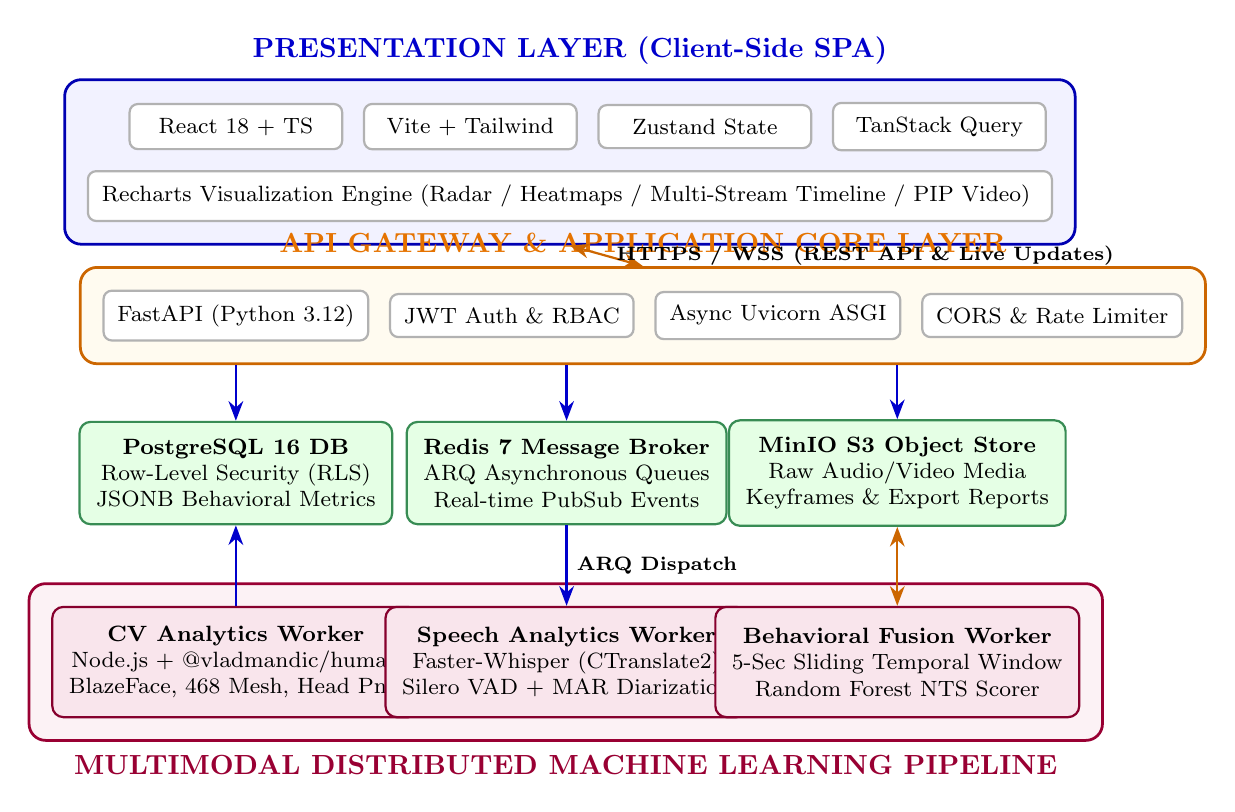
\begin{tikzpicture}[
  node distance=0.4cm and 0.3cm,
  font=\footnotesize,
  compnode/.style={
    draw=gray!60,
    line width=0.8pt,
    rounded corners=3pt,
    fill=white,
    inner sep=5pt,
    align=center,
    font=\footnotesize
  },
  layerbox/.style={
    draw=blue!70!black,
    line width=1pt,
    rounded corners=6pt,
    fill=blue!5,
    inner sep=7pt
  },
  storagenode/.style={
    draw=emerald!70!black,
    line width=0.8pt,
    rounded corners=4pt,
    fill=green!10,
    inner sep=6pt,
    align=center,
    font=\footnotesize
  },
  workernode/.style={
    draw=purple!70!black,
    line width=0.8pt,
    rounded corners=4pt,
    fill=purple!10,
    inner sep=6pt,
    align=center,
    font=\footnotesize
  },
  arrow/.style={-{Stealth[length=2.5mm]}, thick, draw=blue!80!black},
  darrow/.style={{Stealth[length=2.5mm]}-{Stealth[length=2.5mm]}, thick, draw=orange!80!black}
]

% --- LAYER 1: Presentation Layer ---
\node[compnode, minimum width=2.7cm] (c1) at (-4.2, 5.8) {React 18 + TS};
\node[compnode, minimum width=2.7cm, right=0.25cm of c1] (c2) {Vite + Tailwind};
\node[compnode, minimum width=2.7cm, right=0.25cm of c2] (c3) {Zustand State};
\node[compnode, minimum width=2.7cm, right=0.25cm of c3] (c4) {TanStack Query};

\node[compnode, minimum width=12.0cm, below=0.25cm of c2.south east, xshift=-0.1cm] (c5) {
  Recharts Visualization Engine (Radar / Heatmaps / Multi-Stream Timeline / PIP Video)
};

\begin{scope}[on background layer]
  \node[layerbox, fit=(c1) (c4) (c5), inner sep=8pt] (presentation) {};
  \node[above=0.05cm of presentation.north, font=\normalsize\bfseries, text=blue!80!black] {PRESENTATION LAYER (Client-Side SPA)};
\end{scope}

% --- LAYER 2: API Gateway Layer ---
\node[compnode, minimum width=2.7cm] (g1) at (-4.2, 3.4) {FastAPI (Python 3.12)};
\node[compnode, minimum width=2.7cm, right=0.25cm of g1] (g2) {JWT Auth \& RBAC};
\node[compnode, minimum width=2.7cm, right=0.25cm of g2] (g3) {Async Uvicorn ASGI};
\node[compnode, minimum width=2.7cm, right=0.25cm of g3] (g4) {CORS \& Rate Limiter};

\begin{scope}[on background layer]
  \node[layerbox, fill=amber!6, draw=orange!80!black, fit=(g1) (g4), inner sep=8pt] (gateway) {};
  \node[above=0.05cm of gateway.north, font=\normalsize\bfseries, text=orange!90!black] {API GATEWAY \& APPLICATION CORE LAYER};
\end{scope}

% Presentation <-> Gateway connection
\draw[darrow] (presentation.south) -- node[midway, right, font=\scriptsize\bfseries] {HTTPS / WSS (REST API \& Live Updates)} (gateway.north);

% --- LAYER 3: Persistence and Broker ---
\node[storagenode, minimum width=3.6cm, minimum height=1.3cm] (postgres) at (-4.2, 1.4) {
  \textbf{PostgreSQL 16 DB}\\
  Row-Level Security (RLS)\\
  JSONB Behavioral Metrics
};

\node[storagenode, minimum width=3.6cm, minimum height=1.3cm] (redis) at (0, 1.4) {
  \textbf{Redis 7 Message Broker}\\
  ARQ Asynchronous Queues\\
  Real-time PubSub Events
};

\node[storagenode, minimum width=3.6cm, minimum height=1.3cm] (minio) at (4.2, 1.4) {
  \textbf{MinIO S3 Object Store}\\
  Raw Audio/Video Media\\
  Keyframes \& Export Reports
};

\draw[arrow] (gateway.south -| postgres.north) -- (postgres.north);
\draw[arrow] (gateway.south -| redis.north) -- (redis.north);
\draw[arrow] (gateway.south -| minio.north) -- (minio.north);

% --- LAYER 4: ML Processing Layer ---
\node[workernode, minimum width=3.8cm, minimum height=1.4cm] (w_cv) at (-4.2, -1.0) {
  \textbf{CV Analytics Worker}\\
  Node.js + @vladmandic/human\\
  BlazeFace, 468 Mesh, Head PnP
};

\node[workernode, minimum width=3.8cm, minimum height=1.4cm] (w_stt) at (0, -1.0) {
  \textbf{Speech Analytics Worker}\\
  Faster-Whisper (CTranslate2)\\
  Silero VAD + MAR Diarization
};

\node[workernode, minimum width=3.8cm, minimum height=1.4cm] (w_fus) at (4.2, -1.0) {
  \textbf{Behavioral Fusion Worker}\\
  5-Sec Sliding Temporal Window\\
  Random Forest NTS Scorer
};

\begin{scope}[on background layer]
  \node[layerbox, fill=purple!5, draw=purple!80!black, fit=(w_cv) (w_fus), inner sep=8pt] (ml_layer) {};
  \node[below=0.05cm of ml_layer.south, font=\normalsize\bfseries, text=purple!80!black] {MULTIMODAL DISTRIBUTED MACHINE LEARNING PIPELINE};
\end{scope}

% Connections from Storage/Queue to ML Workers
\draw[arrow] (redis.south) -- node[midway, right, font=\scriptsize\bfseries] {ARQ Dispatch} (w_stt.north);
\draw[darrow] (w_fus.north) -- (minio.south);
\draw[arrow] (w_cv.north) -- (postgres.south);

\end{tikzpicture}%
}
\caption{NTS-MIPA System Architecture: Multi-Tier Decoupled Processing Platform}
\label{fig:sysarch}
\end{figure}


As illustrated in Figure~\ref{fig:sysarch}, client interactions originate within a modern Single Page Application (SPA). Multimedia assets (video recordings, live webcam feeds, and CCTV streams) are dispatched via secure multipart HTTPS to the API Gateway. The FastAPI core authenticates user credentials via cryptographic JSON Web Tokens (JWT), verifies project tenancy, and delegates media persistence to an S3-compatible MinIO object storage tier. Concurrently, an asynchronous job record is persisted in PostgreSQL with state set to \texttt{queued}, and an execution task is dispatched to the Redis 7 message broker. Background worker daemons running ARQ (Asynchronous Redis Queue) poll tasks, download localized media chunks, and execute specialized visual, acoustic, and behavioral fusion inference before persisting structured metrics back to PostgreSQL.

\section{FUNCTIONAL REQUIREMENTS}
The functional capabilities of NTS-MIPA are formalized in Table~\ref{tab:functional_reqs}, delineating 18 explicit functional requirements (FR-01 to FR-18) spanning media ingestion, computer vision extraction, acoustic diarization, behavioral inference, and executive reporting.

\begin{table}[htbp]
\centering
\caption{Comprehensive Functional Requirements Specification}
\label{tab:functional_reqs}
\fontsize{8.5}{10.5}\selectfont
\begin{tabularx}{\textwidth}{@{}l p{3.2cm} X@{}}
\toprule
\textbf{Req ID} & \textbf{Requirement Name} & \textbf{Detailed Functional Specification} \\
\midrule
\textbf{FR-01} & Multipart Media Ingestion & The system shall support asynchronous chunked upload of MP4, MKV, and WebM containers up to 4 GB with client-side progress telemetry. \\
\textbf{FR-02} & JWT Authentication & The system shall issue cryptographically signed RS256 JWT access and refresh tokens enforcing Role-Based Access Control (RBAC). \\
\textbf{FR-03} & Video Frame Extraction & The system shall extract normalized JPEG video frames at a configurable sampling rate of 2 FPS via headless FFmpeg worker subprocesses. \\
\textbf{FR-04} & 468-Point Mesh Extraction & The system shall track 468 3D facial landmarks per participant per frame utilizing BlazeFace and MediaPipe topologies. \\
\textbf{FR-05} & Head Pose Kinematics & The system shall compute continuous 3-axis head rotation angles (yaw, pitch, roll) via the Perspective-n-Point (PnP) geometric algorithm. \\
\textbf{FR-06} & Iris Gaze Tracking & The system shall infer ocular gaze vector coordinates for left and right eyes to determine screen-focus and mutual eye-contact duration. \\
\textbf{FR-07} & Affective Classification & The system shall infer a 7-class probability distribution of discrete facial emotions (neutral, happy, sad, angry, surprised, fearful, disgusted). \\
\textbf{FR-08} & Spatial Anchor Tracking & The system shall assign persistent participant identity tracks based on spatial X-axis coordinate clustering to prevent ID swapping. \\
\textbf{FR-09} & Accelerated Speech ASR & The system shall transcribe conversational audio using Faster-Whisper int8 models, generating word-level timestamps and confidence scores. \\
\textbf{FR-10} & Voice Activity Detection & The system shall filter silence and ambient acoustic noise utilizing Silero VAD before dispatching segments to the ASR engine. \\
\textbf{FR-11} & Visual-Acoustic Diarization & The system shall fuse Mouth Aperture Ratio (MAR) with acoustic energy to attribute speech turns accurately during simultaneous cross-talk. \\
\textbf{FR-12} & 5-Second Feature Windowing & The system shall compute rolling 5-second statistical aggregations (mean, variance, entropy) across visual and acoustic telemetry. \\
\textbf{FR-13} & 5-D NTS Regression & The system shall evaluate behavioral vectors via a Random Forest Regressor to output scores ($0-100$) for Communication, Leadership, Engagement, Collaboration, and Confidence. \\
\textbf{FR-14} & Archetype Classification & The system shall classify participants into behavioral archetypes (Presenter, Facilitator, Collaborator, Observer) based on dominant metric centroids. \\
\textbf{FR-15} & Physical CCTV Zone Tracking & The system shall detect and track individuals in overhead CCTV feeds using YOLOv8 and DeepSORT, mapping coordinates to room zones. \\
\textbf{FR-16} & PIP Video Visualization & The frontend shall render synchronized Picture-in-Picture video playback with interactive bounding boxes and gaze direction overlays. \\
\textbf{FR-17} & Interactive Radar Charting & The frontend shall display comparative multi-participant NTS radar diagrams using Recharts with real-time temporal scrub synchronization. \\
\textbf{FR-18} & PDF Coaching Export & The system shall compile and export comprehensive executive coaching summaries in PDF format containing actionable behavioral feedback. \\
\bottomrule
\end{tabularx}
\end{table}

\section{NON-FUNCTIONAL REQUIREMENTS}
System quality attributes, performance constraints, and architectural governance parameters are detailed in Table~\ref{tab:nonfunctional_reqs}.

\begin{table}[htbp]
\centering
\caption{Non-Functional Requirements Specification}
\label{tab:nonfunctional_reqs}
\fontsize{9}{11}\selectfont
\begin{tabularx}{\textwidth}{@{}l p{3.2cm} X@{}}
\toprule
\textbf{NFR ID} & \textbf{Attribute Category} & \textbf{Detailed Engineering Specification} \\
\midrule
\textbf{NFR-01} & Processing Latency & The end-to-end multimodal pipeline shall achieve a Real-Time Factor (RTF) $\le 0.35\times$ on standard GPU hardware (a 60-min meeting processed in $<21$ min). \\
\textbf{NFR-02} & API Response Latency & The API Gateway shall respond to non-inference metadata queries within $\le 120$ milliseconds under a concurrency of 100 simultaneous requests. \\
\textbf{NFR-03} & Horizontal Scalability & Worker daemons shall scale horizontally via containerized Kubernetes pods orchestrated through Redis ARQ task queues without state corruption. \\
\textbf{NFR-04} & Data Isolation \& RLS & Multi-tenant data segregation shall be strictly enforced at the PostgreSQL database engine layer utilizing Row-Level Security (RLS) policies. \\
\textbf{NFR-05} & System Availability & The core REST API and dashboard services shall guarantee a minimum uptime of $99.9\%$ during enterprise operating hours. \\
\textbf{NFR-06} & Cryptographic Security & All data in transit shall be encrypted via TLS 1.3 (HTTPS/WSS), and all persisted multimedia and biometrics in MinIO shall be encrypted at rest (AES-256). \\
\textbf{NFR-07} & Diarization Accuracy & The multimodal speaker diarization module shall maintain a Diarization Error Rate (DER) $\le 10.0\%$ in meeting rooms with up to 6 participants. \\
\textbf{NFR-08} & Cross-Browser Parity & The React frontend SPA shall render deterministically across Google Chrome, Mozilla Firefox, Microsoft Edge, and Apple Safari (desktop viewports $\ge 1280$px). \\
\textbf{NFR-09} & Memory Footprint & Background Node.js CV worker processes shall manage heap allocations dynamically, strictly preventing memory leaks and capping RAM at $\le 2.5$ GB. \\
\textbf{NFR-10} & Extensibility & The system shall expose OpenAPI 3.0 compliant schema endpoints allowing plug-and-play integration with enterprise HRMS systems. \\
\bottomrule
\end{tabularx}
\end{table}

\section{USE CASE DESCRIPTION}
The operational workflows of NTS-MIPA are formalized across five primary use cases:
\begin{enumerate}
    \item \textbf{Use Case UC-1: Secure Meeting Ingestion and Pipeline Enqueueing:}
    \textit{Primary Actor:} Meeting Host / Project Manager.
    \textit{Preconditions:} User is authenticated via JWT and holds project administrative permissions.
    \textit{Workflow:} The user navigates to the meeting creation portal, selects or drags a multi-gigabyte video file, and defines participant identities. The client chunks the binary stream and transmits parts to the FastAPI endpoint \texttt{POST /api/v1/meetings/upload}. The backend verifies the container format via FFprobe, writes the raw binary stream to MinIO, persists a meeting entity in PostgreSQL, enqueues an ARQ task on Redis, and returns an HTTP 202 Accepted status with a unique job UUID.
    
    \item \textbf{Use Case UC-2: Autonomous Multimodal Worker Orchestration:}
    \textit{Primary Actor:} Background ARQ Worker Daemons.
    \textit{Workflow:} The Redis broker dequeues the processing task. The CV worker executes FFmpeg frame extraction at 2 FPS and launches the Node.js \texttt{@vladmandic/human} pipeline, computing facial meshes, gaze vectors, PnP head poses, and emotion vectors. The Audio worker processes the extracted WAV track through Silero VAD and Faster-Whisper, computing word timestamps and pitch dynamics. The Fusion worker executes MAR-assisted diarization and temporal 5-second windowing, invokes the Random Forest NTS model, persists scores in PostgreSQL, and dispatches a WebSocket notification of job completion.

    \item \textbf{Use Case UC-3: Interactive Visual-Acoustic Analytics Exploration:}
    \textit{Primary Actor:} Team Lead / Performance Coach.
    \textit{Workflow:} The user accesses the Meeting Analysis Dashboard. The frontend retrieves normalized telemetry from \texttt{GET /api/v1/meetings/\{id\}/analytics}. The user scrubs through an interactive dual-video player. As the video seeks, synchronized charts dynamically update to show real-time gaze vectors, speaking turns, emotion heatmaps, and NTS metric radar charts for each participant.

    \item \textbf{Use Case UC-4: Physical Conference Room Spatial CCTV Monitoring:}
    \textit{Primary Actor:} Facility Administrator / Organizational Researcher.
    \textit{Workflow:} The system ingests an overhead RTSP or recorded CCTV stream of a physical conference room. The YOLOv8 detector localizes human bounding boxes, while DeepSORT maintains spatial trajectory tracking. Coordinates are projected against pre-calibrated room polygons (Table Zone, Presentation Whiteboard, Exit Zone). The dashboard presents a spatial dwell-time heatmap revealing physical engagement.

    \item \textbf{Use Case UC-5: Automated Executive Coaching Report Generation:}
    \textit{Primary Actor:} Individual Participant / Employee.
    \textit{Workflow:} A participant accesses their private developmental profile via \texttt{GET /api/v1/analytics/coaching/\{user\_id\}}. The system aggregates their individual NTS scores across meetings, compares their radar profile against the organizational benchmark, identifies areas of improvement (e.g., high interruption rate, low gaze stability), and exports an executive PDF development report.
\end{enumerate}

\figplaceholder{NTS-MIPA High-Level Use Case Diagram}{UML Use Case diagram modeling interactions between Meeting Host, Coach, System Administrator, and Background Processing Workers.}

\section{LAYERED ARCHITECTURE DETAIL}
The structural decomposition of NTS-MIPA adheres strictly to separation-of-concerns principles:

\subsection{Presentation Layer}
Constructed as a modern Single Page Application using React 18, TypeScript, and Vite. The user interface leverages Tailwind CSS for responsive styling, Zustand for lightweight client state management, and TanStack React Query for declarative, cached asynchronous server state synchronization. Rich interactive data visualizers are rendered using Recharts, Canvas2D, and HTML5 video primitives.

\subsection{API Gateway and Application Core Layer}
Built using Python 3.12 and FastAPI running on an asynchronous Uvicorn ASGI server. This layer handles SSL termination, CORS negotiation, IP-based rate limiting via Redis token-bucket algorithms, request validation via Pydantic v2 schemas, and cryptographic authorization via JWT and OAuth2 password flows.

\subsection{Asynchronous Task Queue and Message Broker Layer}
Powered by Redis 7 and the ARQ asynchronous framework. Ingestion endpoints push job definitions containing meeting identifiers and processing parameters into high-priority Redis queues. ARQ provides robust task retry logic, exponential backoff, worker dead-letter queues, and real-time pub/sub channels for client WebSocket communication.

\subsection{Multimodal Processing Worker Pool Layer}
A horizontally scalable array of containerized worker daemons:
\begin{itemize}
    \item \textbf{CV Worker:} Executes FFmpeg frame extraction and spawns headless Node.js child processes utilizing \texttt{@vladmandic/human} to perform BlazeFace detection, 468-point facial mesh mapping, Perspective-n-Point (PnP) head pose estimation, and 7-class emotion classification.
    \item \textbf{Speech Worker:} Executes CTranslate2-accelerated Faster-Whisper to generate timestamped phonetic transcripts, calculates pitch fundamental frequency ($F_0$) via autocorrelation, and computes vocal energy.
    \item \textbf{Fusion Worker:} Aligns cross-modal streams into 5-second temporal sliding windows, computes Mouth Aperture Ratio (MAR) cross-correlations, and passes the 32-dimensional behavioral vector to the Random Forest model to compute NTS dimension scores and archetypes.
\end{itemize}

\subsection{Data Persistence and Storage Subsystem}
Comprises two core engines:
\begin{itemize}
    \item \textbf{MinIO Object Storage:} S3-compliant distributed object store housing raw audio-video files, extracted keyframe sequences, and exported coaching dossiers.
    \item \textbf{PostgreSQL 16 Relational Engine:} Houses structured organizational entities, relational associations, user credentials, and time-series behavioral metrics stored in indexed JSONB columns, protected by engine-level Row-Level Security (RLS).
\end{itemize}

\section{DATABASE SCHEMA DESIGN}
The relational database architecture is modeled in Figure~\ref{fig:erdiagram} and detailed in the data dictionary presented in Table~\ref{tab:database_schema}.

\begin{figure}[htbp]
\centering
\resizebox{\linewidth}{!}{%
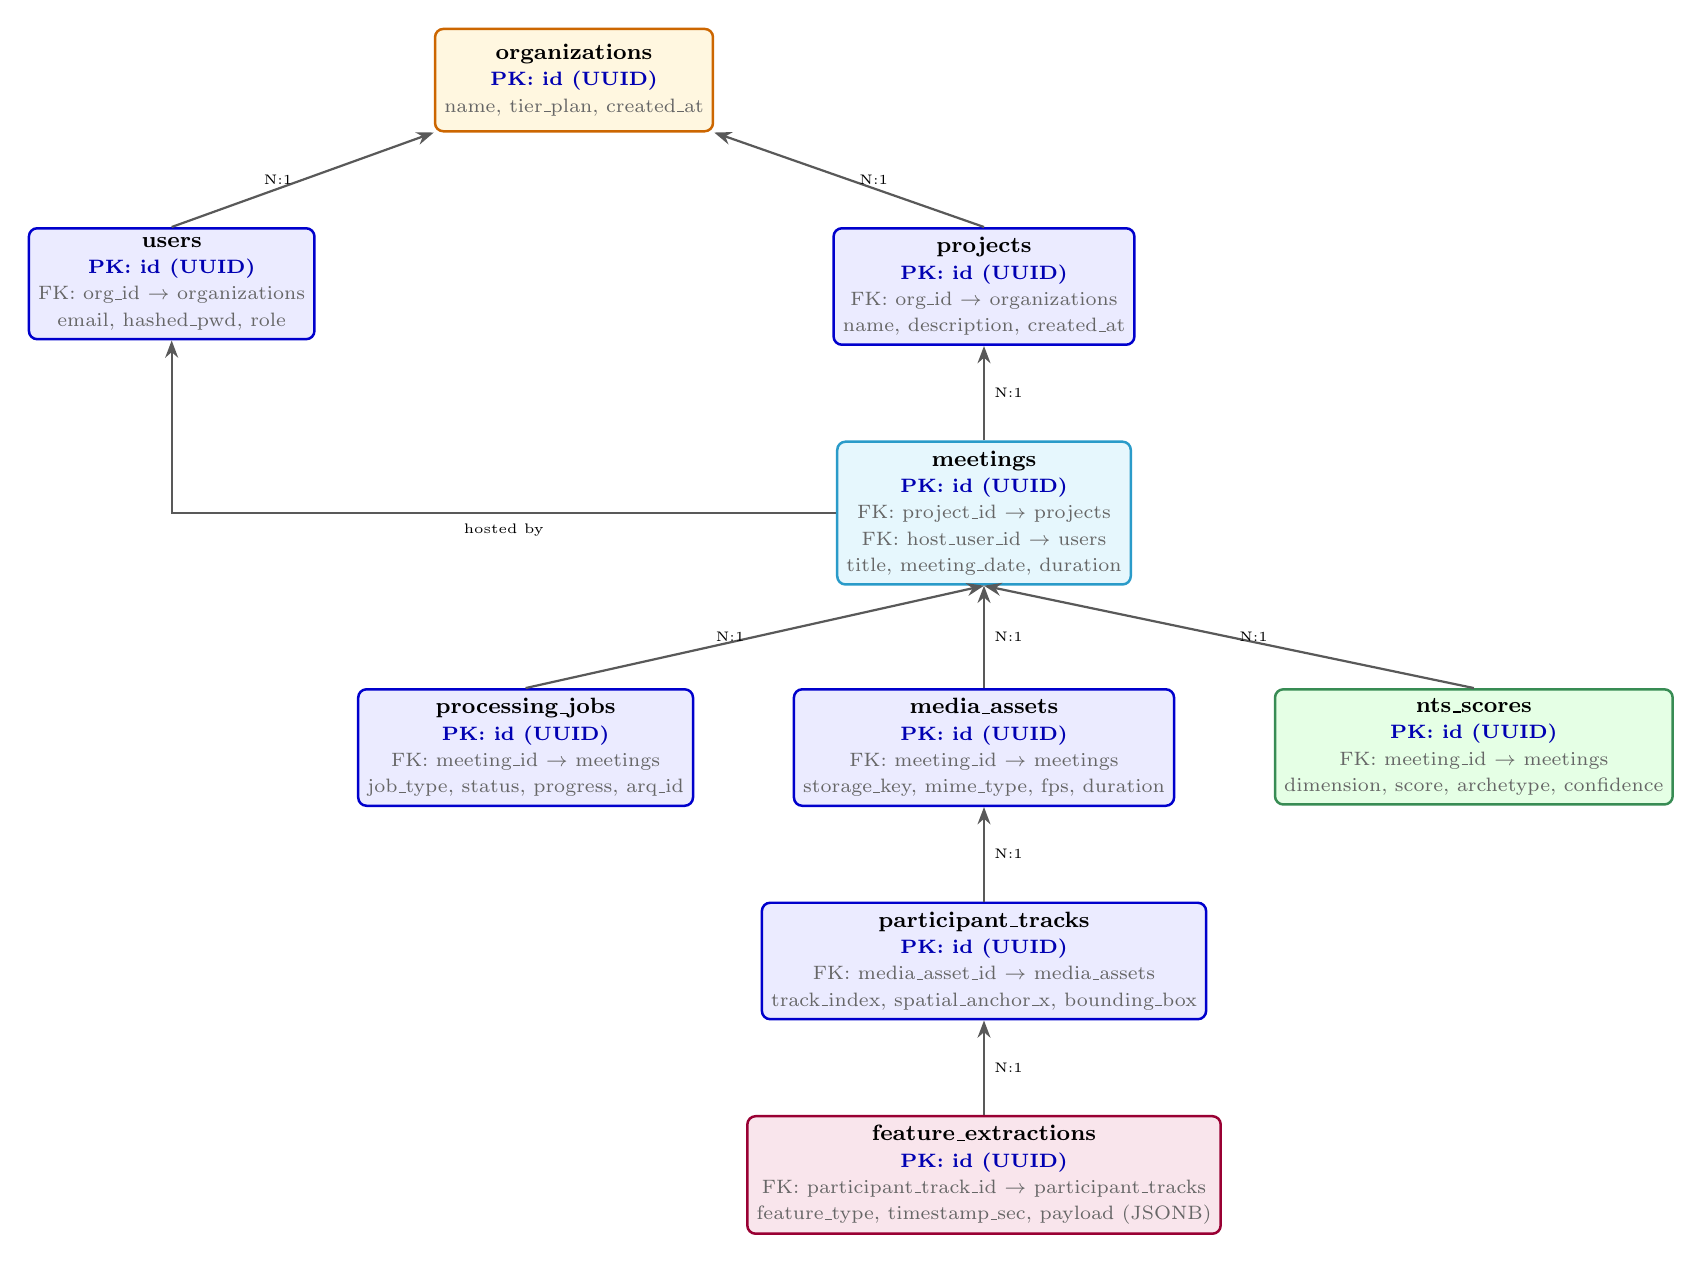
\begin{tikzpicture}[
  font=\footnotesize,
  entity/.style={
    draw=blue!80!black,
    line width=0.9pt,
    rounded corners=3pt,
    fill=blue!8,
    minimum width=3.4cm,
    minimum height=1.3cm,
    align=center,
    font=\footnotesize
  },
  arrow/.style={-{Stealth[length=2.2mm]}, thick, draw=gray!70!black}
]

% Level 1: Organization
\node[entity, fill=amber!12, draw=orange!80!black] (org) at (0, 0) {
  \textbf{organizations}\\
  \pk{PK: id (UUID)}\\
  \fk{name, tier\_plan, created\_at}
};

% Level 2: Users & Projects
\node[entity, below left=1.2cm and 1.5cm of org] (usr) {
  \textbf{users}\\
  \pk{PK: id (UUID)}\\
  \fk{FK: org\_id $\rightarrow$ organizations}\\
  \fk{email, hashed\_pwd, role}
};

\node[entity, below right=1.2cm and 1.5cm of org] (proj) {
  \textbf{projects}\\
  \pk{PK: id (UUID)}\\
  \fk{FK: org\_id $\rightarrow$ organizations}\\
  \fk{name, description, created\_at}
};

\draw[arrow] (usr.north) -- node[midway, left, font=\tiny] {N:1} (org.south west);
\draw[arrow] (proj.north) -- node[midway, right, font=\tiny] {N:1} (org.south east);

% Level 3: Meetings
\node[entity, fill=cyan!10, draw=cyan!80!black, below=1.2cm of proj] (meet) {
  \textbf{meetings}\\
  \pk{PK: id (UUID)}\\
  \fk{FK: project\_id $\rightarrow$ projects}\\
  \fk{FK: host\_user\_id $\rightarrow$ users}\\
  \fk{title, meeting\_date, duration}
};

\draw[arrow] (meet.north) -- node[midway, right, font=\tiny] {N:1} (proj.south);
\draw[arrow] (meet.west) -| node[near start, below, font=\tiny] {hosted by} (usr.south);

% Level 4: Media Assets, Processing Jobs, NTS Scores
\node[entity, below left=1.3cm and 1.8cm of meet] (jobs) {
  \textbf{processing\_jobs}\\
  \pk{PK: id (UUID)}\\
  \fk{FK: meeting\_id $\rightarrow$ meetings}\\
  \fk{job\_type, status, progress, arq\_id}
};

\node[entity, below=1.3cm of meet] (media) {
  \textbf{media\_assets}\\
  \pk{PK: id (UUID)}\\
  \fk{FK: meeting\_id $\rightarrow$ meetings}\\
  \fk{storage\_key, mime\_type, fps, duration}
};

\node[entity, fill=green!10, draw=emerald!70!black, below right=1.3cm and 1.8cm of meet] (nts) {
  \textbf{nts\_scores}\\
  \pk{PK: id (UUID)}\\
  \fk{FK: meeting\_id $\rightarrow$ meetings}\\
  \fk{dimension, score, archetype, confidence}
};

\draw[arrow] (jobs.north) -- node[midway, left, font=\tiny] {N:1} (meet.south);
\draw[arrow] (media.north) -- node[midway, right, font=\tiny] {N:1} (meet.south);
\draw[arrow] (nts.north) -- node[midway, right, font=\tiny] {N:1} (meet.south);

% Level 5: Participant Tracks
\node[entity, below=1.2cm of media] (tracks) {
  \textbf{participant\_tracks}\\
  \pk{PK: id (UUID)}\\
  \fk{FK: media\_asset\_id $\rightarrow$ media\_assets}\\
  \fk{track\_index, spatial\_anchor\_x, bounding\_box}
};

\draw[arrow] (tracks.north) -- node[midway, right, font=\tiny] {N:1} (media.south);

% Level 6: Feature Extractions
\node[entity, fill=purple!10, draw=purple!80!black, below=1.2cm of tracks] (features) {
  \textbf{feature\_extractions}\\
  \pk{PK: id (UUID)}\\
  \fk{FK: participant\_track\_id $\rightarrow$ participant\_tracks}\\
  \fk{feature\_type, timestamp\_sec, payload (JSONB)}
};

\draw[arrow] (features.north) -- node[midway, right, font=\tiny] {N:1} (tracks.south);

\end{tikzpicture}%
}
\caption{Entity-Relationship Schema: Core Database Structure and Behavioral Storage}
\label{fig:erdiagram}
\end{figure}


\begin{table}[htbp]
\centering
\caption{Core Database Relational Entities and Schema Specification}
\label{tab:database_schema}
\fontsize{8.5}{10.5}\selectfont
\begin{tabularx}{\textwidth}{@{}l l l X@{}}
\toprule
\textbf{Table Name} & \textbf{Primary Key} & \textbf{Foreign Keys} & \textbf{Attributes and Data Types} \\
\midrule
\texttt{organizations} & \texttt{id (UUID)} & None & \texttt{name (VARCHAR), plan\_tier (VARCHAR), created\_at (TIMESTAMP)} \\
\addlinespace
\texttt{users} & \texttt{id (UUID)} & \texttt{org\_id $\rightarrow$ organizations} & \texttt{email (VARCHAR), hashed\_password (VARCHAR), role (VARCHAR), full\_name (VARCHAR)} \\
\addlinespace
\texttt{projects} & \texttt{id (UUID)} & \texttt{org\_id $\rightarrow$ organizations} & \texttt{name (VARCHAR), description (TEXT), is\_archived (BOOLEAN)} \\
\addlinespace
\texttt{meetings} & \texttt{id (UUID)} & \texttt{project\_id $\rightarrow$ projects}, \newline \texttt{host\_id $\rightarrow$ users} & \texttt{title (VARCHAR), meeting\_date (DATE), duration\_seconds (INT), status (VARCHAR)} \\
\addlinespace
\texttt{media\_assets} & \texttt{id (UUID)} & \texttt{meeting\_id $\rightarrow$ meetings} & \texttt{storage\_key (VARCHAR), mime\_type (VARCHAR), fps (FLOAT), duration (FLOAT)} \\
\addlinespace
\texttt{processing\_jobs} & \texttt{id (UUID)} & \texttt{meeting\_id $\rightarrow$ meetings} & \texttt{job\_type (VARCHAR), status (VARCHAR), progress (FLOAT), arq\_job\_id (VARCHAR)} \\
\addlinespace
\texttt{participant\_tracks} & \texttt{id (UUID)} & \texttt{media\_asset\_id $\rightarrow$ media\_assets} & \texttt{track\_index (INT), anchor\_x (FLOAT), bounding\_box (JSONB), participant\_name (VARCHAR)} \\
\addlinespace
\texttt{feature\_extractions} & \texttt{id (UUID)} & \texttt{track\_id $\rightarrow$ participant\_tracks} & \texttt{feature\_type (VARCHAR), timestamp\_sec (FLOAT), payload (JSONB)} \\
\addlinespace
\texttt{nts\_scores} & \texttt{id (UUID)} & \texttt{meeting\_id $\rightarrow$ meetings}, \newline \texttt{track\_id $\rightarrow$ participant\_tracks} & \texttt{dimension (VARCHAR), score (FLOAT), confidence (FLOAT), archetype (VARCHAR)} \\
\bottomrule
\end{tabularx}
\end{table}

\section{API DESIGN AND INTERFACE SPECIFICATION}
The system provides a standardized RESTful OpenAPI v3.0 interface. The key endpoint matrix is detailed in Table~\ref{tab:api_endpoints}.

\begin{table}[htbp]
\centering
\caption{RESTful API Core Route Specification}
\label{tab:api_endpoints}
\fontsize{8.5}{10.5}\selectfont
\begin{tabularx}{\textwidth}{@{}l l p{2.2cm} X@{}}
\toprule
\textbf{HTTP Method} & \textbf{Endpoint Path} & \textbf{Auth Required} & \textbf{Functionality and Response Model} \\
\midrule
\texttt{POST} & \texttt{/api/v1/auth/login} & None & Authenticates credentials; returns JWT access/refresh tokens. \\
\texttt{POST} & \texttt{/api/v1/auth/refresh} & Refresh Token & Exchanges valid refresh token for a new short-lived access token. \\
\texttt{POST} & \texttt{/api/v1/meetings/upload} & Bearer JWT & Ingests multipart video container, persists to MinIO, creates job. \\
\texttt{GET}  & \texttt{/api/v1/meetings/\{id\}} & Bearer JWT & Retrieves meeting metadata, duration, status, and participant tracks. \\
\texttt{GET}  & \texttt{/api/v1/meetings/\{id\}/jobs} & Bearer JWT & Polls status and percentage completion of asynchronous ML jobs. \\
\texttt{GET}  & \texttt{/api/v1/meetings/\{id\}/analytics} & Bearer JWT & Returns consolidated 5-D NTS scores, archetypes, and metrics. \\
\texttt{GET}  & \texttt{/api/v1/meetings/\{id\}/timeline} & Bearer JWT & Returns synchronized 1-second timeseries of gaze, emotion, speech. \\
\texttt{GET}  & \texttt{/api/v1/meetings/\{id\}/cctv} & Bearer JWT & Returns spatial room tracking coordinates and zone dwell times. \\
\texttt{POST} & \texttt{/api/v1/meetings/\{id\}/export} & Bearer JWT & Generates downloadable executive coaching PDF evaluation. \\
\bottomrule
\end{tabularx}
\end{table}

\figplaceholder{NTS-MIPA Architectural Data Flow Diagram}{Detailed DFD illustrating Level-1 data flows between React client, API Gateway, Redis Queue, ML Workers, and PostgreSQL database.}

\chapter{IMPLEMENTATION DETAILS}

\section{DEVELOPMENT ENVIRONMENT AND TOOLCHAIN}
The implementation of NTS-MIPA spans a modern, containerized full-stack architecture orchestrated across Python, TypeScript, Node.js, and CUDA-accelerated native runtimes. The development stack versions and hardware infrastructure utilized for engineering and evaluating the platform are summarized in Table~\ref{tab:dev_environment}.

\begin{table}[htbp]
\centering
\caption{System Toolchain and Execution Environment Specifications}
\label{tab:dev_environment}
\fontsize{9}{11}\selectfont
\begin{tabularx}{\textwidth}{@{}l p{4.2cm} X@{}}
\toprule
\textbf{Subsystem Layer} & \textbf{Technology / Library} & \textbf{Version and Operational Configuration} \\
\midrule
\textbf{Host OS} & Ubuntu Linux 22.04 LTS / Windows 11 & Linux Kernel 6.5 / WSL2 with CUDA 12.2 \\
\textbf{Compute Acceleration} & NVIDIA CUDA Toolkit \& cuDNN & CUDA 12.2, cuDNN 8.9.4 on NVIDIA RTX 4070 (8 GB) \\
\textbf{Backend Runtime} & Python 3.12.3 & Asynchronous runtime via \texttt{asyncio} and Uvicorn \\
\textbf{Web API Framework} & FastAPI & Version 0.111.0 with Pydantic v2 data validation \\
\textbf{Database Engine} & PostgreSQL & Version 16.2 with native JSONB indexing and RLS \\
\textbf{Cache \& Message Broker} & Redis \& ARQ & Redis 7.2-alpine, ARQ 0.25.0 asynchronous queue \\
\textbf{Object Storage} & MinIO (S3 Compatible) & RELEASE.2024-04-18T19-09-19Z \\
\textbf{Media Processing} & FFmpeg \& FFprobe & Version 6.1.1 static multi-threaded builds \\
\textbf{CV Runtime} & Node.js \& @vladmandic/human & Node v20.12.2, @vladmandic/human v3.2.3 (TensorFlow.js) \\
\textbf{ASR Inference Engine} & Faster-Whisper & Version 1.0.1 running on CTranslate2 int8 \\
\textbf{Spatial Tracker} & Ultralytics YOLOv8 \& DeepSORT & YOLOv8m (PyTorch 2.3.0), deep-sort-realtime 1.3.2 \\
\textbf{ML Regressor} & Scikit-Learn & Version 1.4.2 (RandomForestRegressor, joblib) \\
\textbf{Frontend Framework} & React 18, Vite, TypeScript & React 18.3.1, TypeScript 5.4.5, Vite 5.2.11 \\
\textbf{Styling \& UI Library} & Tailwind CSS, Lucide React & Tailwind v3.4.3, Lucide-react v0.378.0 \\
\textbf{State \& Visuals} & Zustand, TanStack Query, Recharts & Zustand 4.5.2, React Query 5.35.1, Recharts 2.12.7 \\
\bottomrule
\end{tabularx}
\end{table}

\section{BACKEND INFRASTRUCTURE AND AUTHENTICATION}
The backend service is structured as an asynchronous FastAPI application. Authentication is handled using asymmetric cryptographic JSON Web Tokens (JWT) enforcing Role-Based Access Control (RBAC). 

\subsection{JWT Authentication and Password Hashing}
The authentication pipeline utilizes \texttt{passlib} with the BCrypt hashing scheme (12 computational rounds). Upon successful credential verification, the system issues a short-lived access token (valid for 30 minutes) and a long-lived cryptographically signed refresh token (valid for 7 days) persisted in an HttpOnly, SameSite-strict cookie to prevent cross-site scripting (XSS) attacks. Listing~\ref{lst:auth_code} shows the production implementation of the login endpoint.

\begin{lstlisting}[language=Python, caption={FastAPI Authentication and JWT Token Issuance Routine}, label={lst:auth_code}]
@router.post("/login", response_model=TokenResponse)
async def login(
    data: LoginRequest, 
    response: Response, 
    db: AsyncSession = Depends(get_db)
):
    user = await user_service.authenticate(db, data.email, data.password)
    if not user:
        raise HTTPException(
            status_code=status.HTTP_401_UNAUTHORIZED, 
            detail="Invalid credentials provided."
        )
    
    access_token = security.create_access_token(
        data={"sub": str(user.id), "org_id": str(user.org_id), "role": user.role}
    )
    refresh_token = security.create_refresh_token(
        data={"sub": str(user.id)}
    )
    
    await auth_service.store_refresh_token(db, user.id, refresh_token)
    response.set_cookie(
        key="refresh_token", 
        value=refresh_token, 
        httponly=True, 
        secure=True, 
        samesite="lax"
    )
    return TokenResponse(access_token=access_token, token_type="bearer")
\end{lstlisting}

\subsection{Asynchronous Job Enqueueing with ARQ}
To ensure zero degradation of REST API response times, heavy machine learning pipelines are orchestrated via ARQ and Redis. Listing~\ref{lst:arq_code} illustrates the non-blocking job submission routine that persists the job entity to PostgreSQL and enqueues the task ID into Redis.

\begin{lstlisting}[language=Python, caption={Asynchronous Redis Task Enqueueing with ARQ}, label={lst:arq_code}]
async def enqueue_analysis(
    db: AsyncSession, 
    meeting_id: UUID, 
    pipeline_type: str = "full_multimodal"
) -> ProcessingJob:
    job = ProcessingJob(
        meeting_id=meeting_id,
        job_type=pipeline_type,
        status="queued",
        progress=0.0,
        priority=10
    )
    db.add(job)
    await db.flush()
    
    # Enqueue job into Redis pool with meeting parameters
    arq_job = await redis_pool.enqueue_job(
        "process_meeting_pipeline", 
        meeting_id=str(meeting_id), 
        job_id=str(job.id)
    )
    job.arq_job_id = arq_job.job_id
    await db.commit()
    return job
\end{lstlisting}

\section{COMPUTER VISION PIPELINE AND TRACKING}
The computer vision subsystem processes meeting video streams to quantify fine-grained human facial kinetics, gaze directions, and emotional states without requiring manual participant tagging. The complete multi-stage computer vision workflow is depicted in Figure~\ref{fig:cvpipeline}.

\begin{figure}[htbp]
\centering
\resizebox{\linewidth}{!}{%
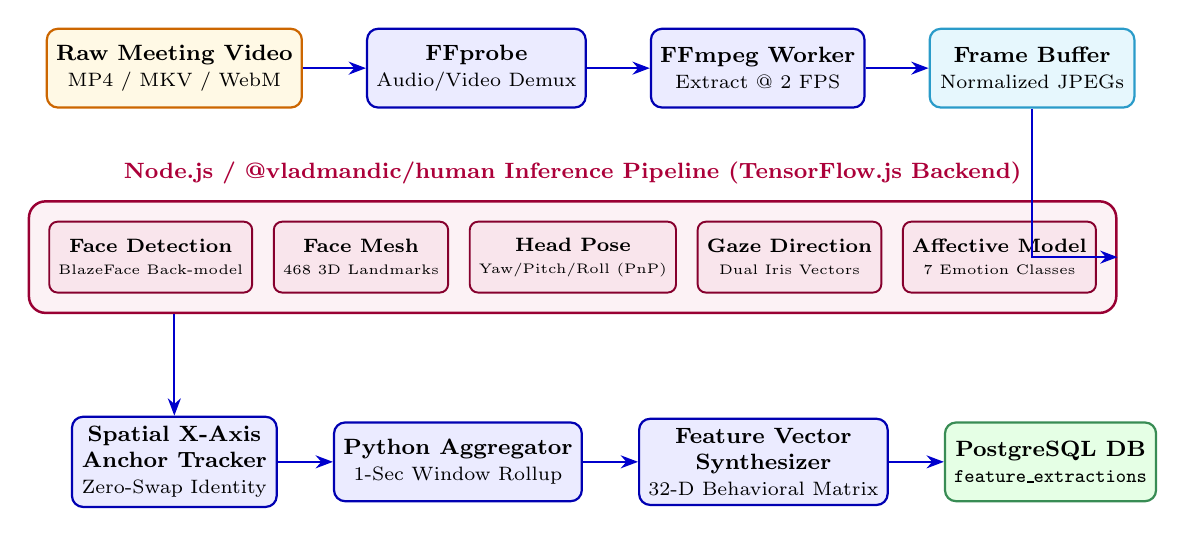
\begin{tikzpicture}[
  font=\footnotesize,
  block/.style={
    draw=blue!70!black,
    line width=0.8pt,
    rounded corners=4pt,
    fill=blue!8,
    minimum width=2.6cm,
    minimum height=1cm,
    align=center,
    font=\footnotesize
  },
  subblock/.style={
    draw=purple!70!black,
    line width=0.7pt,
    rounded corners=3pt,
    fill=purple!10,
    minimum width=2.2cm,
    minimum height=0.9cm,
    align=center,
    font=\scriptsize
  },
  storage/.style={
    draw=emerald!70!black,
    line width=0.8pt,
    rounded corners=4pt,
    fill=green!10,
    minimum width=2.6cm,
    minimum height=1cm,
    align=center,
    font=\footnotesize
  },
  arrow/.style={-{Stealth[length=2.2mm]}, thick, draw=blue!80!black}
]

% First row: Video Input & FFmpeg
\node[block, fill=amber!10, draw=orange!80!black] (video) at (-4.5, 3.2) {\textbf{Raw Meeting Video}\\\scriptsize MP4 / MKV / WebM};
\node[block, right=0.8cm of video] (ffprobe) {\textbf{FFprobe}\\\scriptsize Audio/Video Demux};
\node[block, right=0.8cm of ffprobe] (ffmpeg) {\textbf{FFmpeg Worker}\\\scriptsize Extract @ 2 FPS};
\node[block, fill=cyan!10, draw=cyan!80!black, right=0.8cm of ffmpeg] (frames) {\textbf{Frame Buffer}\\\scriptsize Normalized JPEGs};

\draw[arrow] (video) -- (ffprobe);
\draw[arrow] (ffprobe) -- (ffmpeg);
\draw[arrow] (ffmpeg) -- (frames);

% Second row: Individual Human.js inference stages
\node[subblock] (f1) at (-4.8, 0.8) {\textbf{Face Detection}\\\tiny BlazeFace Back-model};
\node[subblock, right=0.25cm of f1] (f2) {\textbf{Face Mesh}\\\tiny 468 3D Landmarks};
\node[subblock, right=0.25cm of f2] (f3) {\textbf{Head Pose}\\\tiny Yaw/Pitch/Roll (PnP)};
\node[subblock, right=0.25cm of f3] (f4) {\textbf{Gaze Direction}\\\tiny Dual Iris Vectors};
\node[subblock, right=0.25cm of f4] (f5) {\textbf{Affective Model}\\\tiny 7 Emotion Classes};

\begin{scope}[on background layer]
  \node[draw=purple!80!black, fill=purple!5, rounded corners=6pt, line width=0.9pt, fit=(f1) (f5), inner sep=7pt] (human_box) {};
  \node[above=0.08cm of human_box.north, font=\footnotesize\bfseries, text=purple!90!black] {Node.js / @vladmandic/human Inference Pipeline (TensorFlow.js Backend)};
\end{scope}

\draw[arrow] (frames.south) |- (human_box.east);

% Third row: Tracking, Aggregation, and Storage
\node[block] (anchor) at (-4.5, -1.8) {\textbf{Spatial X-Axis}\\\textbf{Anchor Tracker}\\\scriptsize Zero-Swap Identity};
\node[block, right=0.7cm of anchor] (aggregator) {\textbf{Python Aggregator}\\\scriptsize 1-Sec Window Rollup};
\node[block, right=0.7cm of aggregator] (features) {\textbf{Feature Vector}\\\textbf{Synthesizer}\\\scriptsize 32-D Behavioral Matrix};
\node[storage, right=0.7cm of features] (db) {\textbf{PostgreSQL DB}\\\scriptsize \texttt{feature\_extractions}};

\draw[arrow] (human_box.south -| anchor.north) -- (anchor.north);
\draw[arrow] (anchor) -- (aggregator);
\draw[arrow] (aggregator) -- (features);
\draw[arrow] (features) -- (db);

\end{tikzpicture}%
}
\caption{Computer Vision Multi-Stage Behavioral Extraction Pipeline}
\label{fig:cvpipeline}
\end{figure}


\subsection{Node.js and @vladmandic/human Integration}
Video files are initially processed via multi-threaded FFmpeg subprocesses to extract normalized JPEG frames at 2 frames per second (FPS). A dedicated Node.js service utilizes \texttt{@vladmandic/human} to process frame batches. The inference script configures TensorFlow.js with direct hardware acceleration, enabling BlazeFace detection, 468-point 3D landmark mesh construction, and 7-class emotion probabilities. Listing~\ref{lst:human_js} illustrates the core Node.js execution handler.

\begin{lstlisting}[language=Java, caption={Headless Node.js Human.js Computer Vision Extraction Handler}, label={lst:human_js}]
import { Human } from '@vladmandic/human';
import fs from 'fs';

const humanConfig = {
  backend: 'tensorflow',
  modelBasePath: 'file://./models',
  face: {
    enabled: true,
    detector: { modelPath: 'blazeface.json', maxDetected: 10, minConfidence: 0.5 },
    mesh: { enabled: true, modelPath: 'facemesh.json' },
    iris: { enabled: true, modelPath: 'iris.json' },
    emotion: { enabled: true, modelPath: 'emotion.json' },
    description: { enabled: false }
  },
  body: { enabled: false },
  hand: { enabled: false }
};

const human = new Human(humanConfig);

export async function processFrame(framePath) {
  const buffer = fs.readFileSync(framePath);
  const tensor = human.tf.node.decodeImage(buffer, 3);
  const result = await human.detect(tensor);
  human.tf.dispose(tensor);
  
  return result.face.map(f => ({
    box: f.box,
    score: f.score,
    rotation: f.rotation, // [yaw, pitch, roll] in radians via PnP
    gaze: f.gaze,         // Normalized bearing vector [x, y]
    emotions: f.emotion,  // [{ score, emotion: 'neutral'|'happy'|... }]
    mesh: f.mesh          // 468 [x, y, z] normalized coordinates
  }));
}
\end{lstlisting}

\subsection{Head Pose Estimation via Perspective-n-Point (PnP)}
To infer 3D head rotation from a monocular 2D video feed, the system formulates the classical Perspective-n-Point (PnP) problem \parencite{lepetit2009epnp}. Using six canonical 3D facial feature points (nose tip, chin, left eye corner, right eye corner, left mouth corner, right mouth corner) mapped against standard Anthropometric 3D facial models, the rotation matrix $\mathbf{R} \in \mathbb{SO}(3)$ and translation vector $\mathbf{t} \in \mathbb{R}^3$ are solved:
\begin{equation}
    s \begin{bmatrix} u \\ v \\ 1 \end{bmatrix} = \mathbf{K} \begin{bmatrix} \mathbf{R} & \mathbf{t} \end{bmatrix} \begin{bmatrix} X_w \\ Y_w \\ Z_w \\ 1 \end{bmatrix}
\end{equation}
where $\mathbf{K}$ represents the intrinsic pinhole camera matrix:
\begin{equation}
    \mathbf{K} = \begin{bmatrix} f_x & 0 & c_x \\ 0 & f_y & c_y \\ 0 & 0 & 1 \end{bmatrix}
\end{equation}
The rotation matrix $\mathbf{R}$ is decomposed into Euler angles producing head Yaw ($\psi$), Pitch ($\theta$), and Roll ($\phi$).

\subsection{Spatial X-Axis Anchor Tracking Algorithm}
In standard conference room geometries, participants remain seated in fixed relative horizontal positions along the meeting table. Because DeepSORT's deep appearance descriptors frequently trigger identity switches when participants turn their heads laterally, NTS-MIPA introduces the \textbf{Spatial X-Axis Anchor Tracking} algorithm. The algorithm clusters normalized horizontal bounding box centroids ($c_{x,i} \in [0, 1]$) across the initial $N_{\text{init}}$ calibration frames to establish fixed spatial anchors $\mathcal{A} = \{a_1, a_2, \dots, a_K\}$ where $a_1 < a_2 < \dots < a_K$. In subsequent frames, detected faces are assigned to the nearest spatial anchor using a 1D Hungarian matching cost matrix constrained by an empirical drift threshold $\tau = 0.08$.

\begin{lstlisting}[language=Python, caption={Spatial X-Axis Anchor Tracking Algorithm Pseudocode}, label={lst:anchor_tracking}]
def initialize_spatial_anchors(calibration_detections: list, K_participants: int):
    # Collect all normalized X-center coordinates over initial 5 seconds
    x_centers = [det.box[0] + (det.box[2] / 2.0) for det in calibration_detections]
    kmeans = KMeans(n_clusters=K_participants, n_init=10).fit(np.array(x_centers).reshape(-1, 1))
    anchors = np.sort(kmeans.cluster_centers_.flatten())
    return anchors

def assign_detections_to_tracks(detections: list, anchors: np.ndarray, drift_thresh: float = 0.08):
    assigned_tracks = {}
    det_x = np.array([d.box[0] + (d.box[2] / 2.0) for d in detections])
    
    # Compute Euclidean cost matrix between detections and spatial anchors
    cost_matrix = np.abs(det_x[:, np.newaxis] - anchors[np.newaxis, :])
    row_ind, col_ind = scipy.optimize.linear_sum_assignment(cost_matrix)
    
    for r, c in zip(row_ind, col_ind):
        if cost_matrix[r, c] <= drift_thresh:
            assigned_tracks[c] = detections[r]  # Anchor 'c' deterministically assigned
        else:
            handle_temporary_occlusion(c)
    return assigned_tracks
\end{lstlisting}

\figplaceholder{Sample Meeting Frame with Bounding Box and 468-Mesh Overlay}{Annotated conference frame depicting BlazeFace bounding boxes, head pose vectors, and iris gaze points.}

\section{SPEECH AND AUDIO PROCESSING}
Audio processing operates in parallel with computer vision, extracting linguistic transcripts and vocal prosodic signals.

\subsection{Faster-Whisper Integration and VAD}
The raw audio track is demuxed into a 16 kHz single-channel linear PCM WAV file. Silero VAD is applied with a speech probability threshold of $0.5$ to eliminate non-speech acoustic segments. Surviving speech audio chunks are ingested by Faster-Whisper configured with CTranslate2 int8 execution on GPU. Listing~\ref{lst:whisper_code} displays the transcription extraction routine.

\begin{lstlisting}[language=Python, caption={Accelerated Speech-to-Text Transcription via Faster-Whisper}, label={lst:whisper_code}]
from faster_whisper import WhisperModel

model = WhisperModel("base.en", device="cuda", compute_type="int8")

def transcribe_audio_stream(audio_path: str):
    segments, info = model.transcribe(
        audio_path,
        beam_size=5,
        word_timestamps=True,
        vad_filter=True,
        vad_parameters=dict(min_silence_duration_ms=500)
    )
    
    transcriptions = []
    for segment in segments:
        for word in segment.words:
            transcriptions.append({
                "word": word.word.strip(),
                "start": word.start,
                "end": word.end,
                "confidence": word.probability
            })
    return transcriptions
\end{lstlisting}

\subsection{Mouth Aperture Ratio (MAR) Visual Diarization Fusion}
To resolve acoustic speaker attribution when multiple participants speak simultaneously, NTS-MIPA correlates acoustic speech segments with visual lip aperture dynamics. Utilizing MediaPipe's 468-point facial mesh, the \textbf{Mouth Aperture Ratio (MAR)} is computed from the vertical inner lip landmarks (top lip 13, bottom lip 14) and horizontal mouth corners (left corner 78, right corner 308):
\begin{equation}
    \text{MAR} = \frac{\|\mathbf{p}_{13} - \mathbf{p}_{14}\|_2}{\|\mathbf{p}_{78} - \mathbf{p}_{308}\|_2 + \epsilon}
\end{equation}
where $\epsilon = 10^{-7}$ prevents division by zero. A participant is classified as actively vocalizing if $\text{MAR}(t) \ge \tau_{\text{mouth}} = 0.18$ across consecutive frames, matching the acoustic onset. Listing~\ref{lst:mar_code} provides the implementation.

\begin{lstlisting}[language=Python, caption={Mouth Aperture Ratio (MAR) Calculation from Facial Landmarks}, label={lst:mar_code}]
def compute_mar(landmarks: list) -> float:
    """Computes Mouth Aperture Ratio (MAR) using MediaPipe inner-lip coordinates."""
    top_lip = landmarks[13]      # Upper inner lip center
    bottom_lip = landmarks[14]   # Lower inner lip center
    left_corner = landmarks[78]  # Left oral commissure
    right_corner = landmarks[308]# Right oral commissure
    
    vertical = np.linalg.norm(
        np.array([top_lip.x - bottom_lip.x, top_lip.y - bottom_lip.y, top_lip.z - bottom_lip.z])
    )
    horizontal = np.linalg.norm(
        np.array([left_corner.x - right_corner.x, left_corner.y - right_corner.y, left_corner.z - right_corner.z])
    )
    return float(vertical / (horizontal + 1e-7))
\end{lstlisting}

\figplaceholder{Mouth Aperture Ratio Lip Dynamics Tracking Overlay}{Visualization of the 468-point mesh inner lip distance tracking vocal articulation during conversation.}

\section{FEATURE FUSION AND NTS SCORING ENGINE}
The behavioral scoring engine maps multimodal telemetry into standardized non-technical skill metrics. The complete inference pipeline is illustrated in Figure~\ref{fig:ntspipeline}.

\begin{figure}[htbp]
\centering
\resizebox{\linewidth}{!}{%
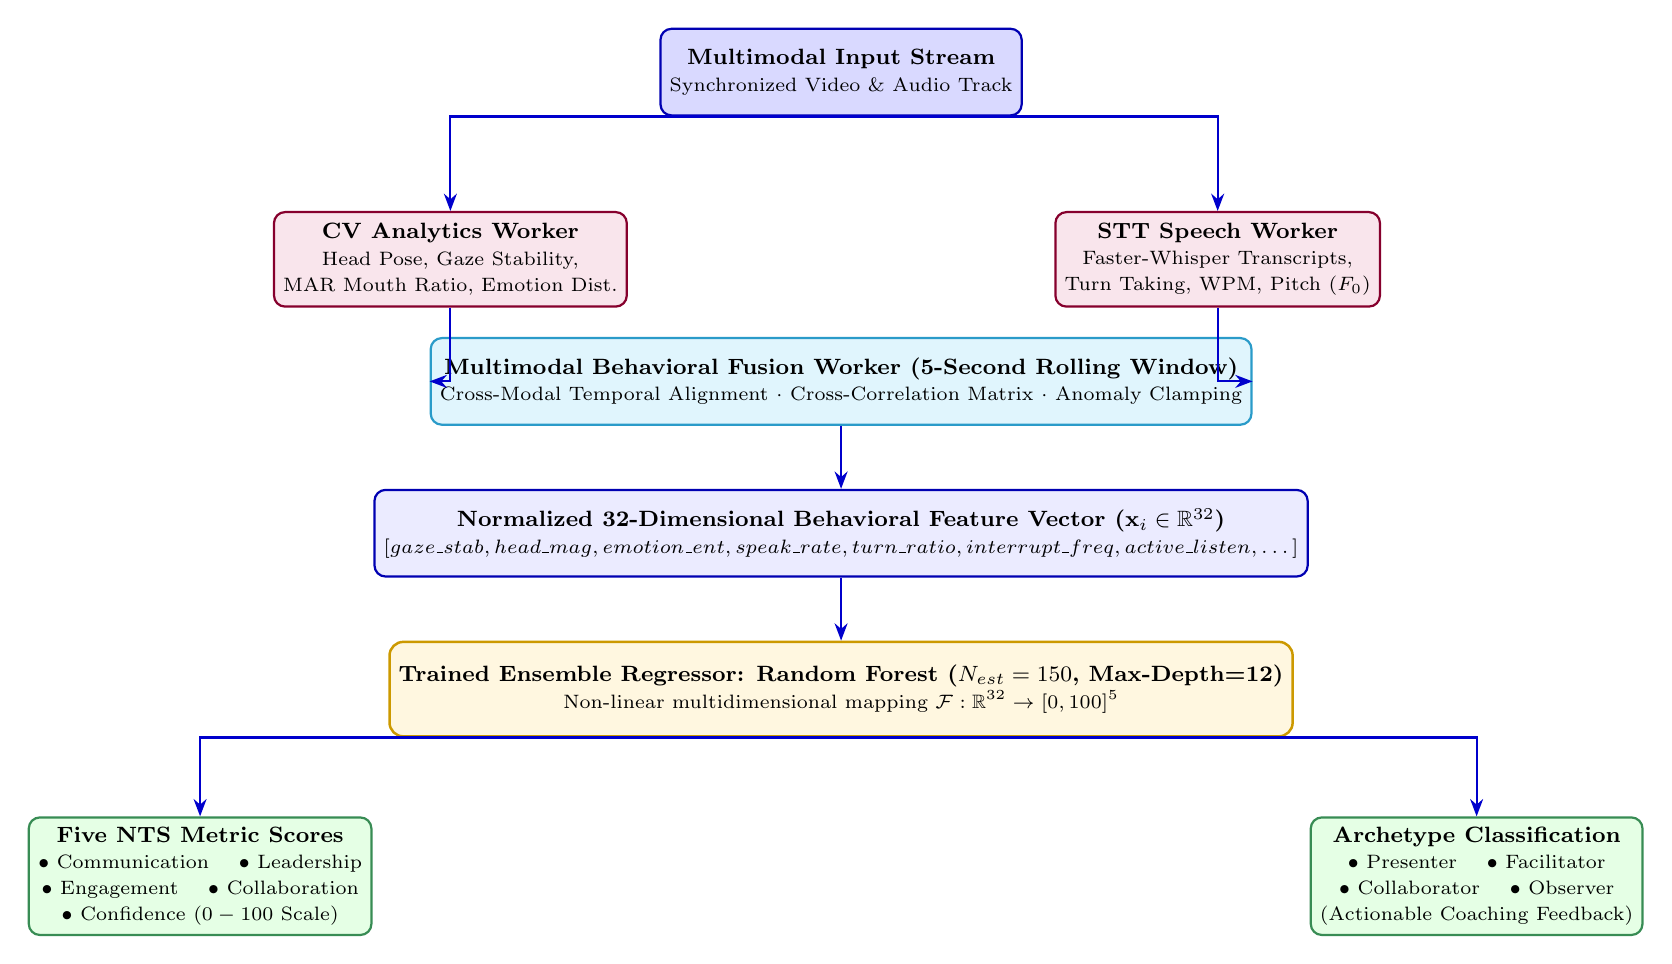
\begin{tikzpicture}[
  font=\footnotesize,
  block/.style={
    draw=blue!70!black,
    line width=0.8pt,
    rounded corners=4pt,
    fill=blue!8,
    minimum width=3.2cm,
    minimum height=1.1cm,
    align=center,
    font=\footnotesize
  },
  worker/.style={
    draw=purple!70!black,
    line width=0.8pt,
    rounded corners=4pt,
    fill=purple!10,
    minimum width=3.4cm,
    minimum height=1.2cm,
    align=center,
    font=\footnotesize
  },
  modelnode/.style={
    draw=amber!80!black,
    line width=0.9pt,
    rounded corners=5pt,
    fill=amber!12,
    minimum width=3.8cm,
    minimum height=1.2cm,
    align=center,
    font=\footnotesize
  },
  outnode/.style={
    draw=emerald!70!black,
    line width=0.8pt,
    rounded corners=4pt,
    fill=green!10,
    minimum width=3.4cm,
    minimum height=1.2cm,
    align=center,
    font=\footnotesize
  },
  arrow/.style={-{Stealth[length=2.2mm]}, thick, draw=blue!80!black}
]

% Input
\node[block, fill=blue!15] (input) at (0,0) {\textbf{Multimodal Input Stream}\\\scriptsize Synchronized Video \& Audio Track};

% Two workers
\node[worker, below left=1.2cm and 0.4cm of input] (cv_worker) {
  \textbf{CV Analytics Worker}\\
  \scriptsize Head Pose, Gaze Stability,\\
  \scriptsize MAR Mouth Ratio, Emotion Dist.
};

\node[worker, below right=1.2cm and 0.4cm of input] (stt_worker) {
  \textbf{STT Speech Worker}\\
  \scriptsize Faster-Whisper Transcripts,\\
  \scriptsize Turn Taking, WPM, Pitch ($F_0$)
};

\draw[arrow] (input.south) -| (cv_worker.north);
\draw[arrow] (input.south) -| (stt_worker.north);

% Fusion Worker
\node[block, fill=cyan!12, draw=cyan!80!black, minimum width=8.5cm, below=1.2cm of input, yshift=-1.6cm] (fusion) {
  \textbf{Multimodal Behavioral Fusion Worker (5-Second Rolling Window)}\\
  \scriptsize Cross-Modal Temporal Alignment $\cdot$ Cross-Correlation Matrix $\cdot$ Anomaly Clamping
};

\draw[arrow] (cv_worker.south) |- (fusion.west);
\draw[arrow] (stt_worker.south) |- (fusion.east);

% Feature Vector
\node[block, minimum width=8.5cm, below=0.8cm of fusion] (fvec) {
  \textbf{Normalized 32-Dimensional Behavioral Feature Vector ($\mathbf{x}_i \in \mathbb{R}^{32}$)}\\
  \scriptsize $[gaze\_stab, head\_mag, emotion\_ent, speak\_rate, turn\_ratio, interrupt\_freq, active\_listen, \dots]$
};

\draw[arrow] (fusion) -- (fvec);

% ML Model
\node[modelnode, minimum width=8.5cm, below=0.8cm of fvec] (rf_model) {
  \textbf{Trained Ensemble Regressor: Random Forest ($N_{est}=150$, Max-Depth=12)}\\
  \scriptsize Non-linear multidimensional mapping $\mathcal{F}: \mathbb{R}^{32} \rightarrow [0, 100]^5$
};

\draw[arrow] (fvec) -- (rf_model);

% Outputs
\node[outnode, below left=1.0cm and 0.2cm of rf_model] (nts_scores) {
  \textbf{Five NTS Metric Scores}\\
  \scriptsize $\bullet$ Communication $\quad \bullet$ Leadership\\
  \scriptsize $\bullet$ Engagement $\quad \bullet$ Collaboration\\
  \scriptsize $\bullet$ Confidence ($0 - 100$ Scale)
};

\node[outnode, below right=1.0cm and 0.2cm of rf_model] (archetypes) {
  \textbf{Archetype Classification}\\
  \scriptsize $\bullet$ Presenter $\quad \bullet$ Facilitator\\
  \scriptsize $\bullet$ Collaborator $\quad \bullet$ Observer\\
  \scriptsize (Actionable Coaching Feedback)
};

\draw[arrow] (rf_model.south) -| (nts_scores.north);
\draw[arrow] (rf_model.south) -| (archetypes.north);

\end{tikzpicture}%
}
\caption{Multimodal Non-Technical Skills (NTS) Scoring and Behavioral Inference Pipeline}
\label{fig:ntspipeline}
\end{figure}


\subsection{Temporal Sliding Window Aggregation}
Visual features (2 FPS) and acoustic features are aligned into rolling 5-second temporal windows with a 1-second step size ($80\%$ overlap). For each participant $k$ in window $w$, the system constructs a 32-dimensional behavioral feature vector $\mathbf{x}_{k,w} \in \mathbb{R}^{32}$:
\begin{itemize}
    \item \textbf{Visual Kinematic Features (12):} Gaze stability index, mean yaw angular velocity, pitch nodding frequency, roll tilt variance, blink frequency, facial motion energy.
    \item \textbf{Affective Features (7):} 7-class normalized emotion entropy:
    \begin{equation}
        H_{\text{emo}} = -\sum_{i=1}^7 p_i \log_2(p_i + \epsilon)
    \end{equation}
    \item \textbf{Conversational Acoustic Features (8):} Speaking rate in Words Per Minute (WPM), speech turn duration, turn-taking ratio, interruption initiation count, backchannel feedback frequency, vocal pitch mean ($\mu_{F_0}$), pitch variance ($\sigma_{F_0}$).
    \item \textbf{Interpersonal Coordination Features (5):} Mutual gaze convergence ratio, cross-participant head nod mimicry, conversational latency (response gap in seconds).
\end{itemize}

\subsection{Ensemble Random Forest NTS Regressor}
To model the non-linear, non-monotonic mapping between behavioral features and non-technical skills, an ensemble \textbf{Random Forest Regressor} \parencite{breiman2001random, pedregosa2011scikit} parameterized with 150 estimator trees and a maximum tree depth of 12 was trained on expert-annotated meeting benchmarks. Listing~\ref{lst:rf_scoring} presents the scoring evaluation routine.

\begin{lstlisting}[language=Python, caption={Random Forest NTS Metric Scoring Routine}, label={lst:rf_scoring}]
def score_participant_behavior(features: dict, rf_regressor) -> NTSMetricScore:
    """Evaluates 32-dimensional behavioral feature vector via Random Forest."""
    feature_vector = np.array([
        features.get("gaze_stability", 0.0),
        features.get("head_motion_magnitude", 0.0),
        features.get("emotion_entropy", 0.0),
        features.get("speaking_rate_wpm", 0.0),
        features.get("turn_taking_ratio", 0.0),
        features.get("interruption_rate", 0.0),
        features.get("listening_engagement", 0.0),
        features.get("mutual_gaze_ratio", 0.0),
        features.get("pitch_variability", 0.0),
        # ... remaining 23 normalized behavioral dimensions
    ]).reshape(1, -1)
    
    # Predict multi-output continuous regression vector in range [0, 100]
    scores = rf_regressor.predict(feature_vector)[0]
    
    return NTSMetricScore(
        communication=round(float(np.clip(scores[0], 0, 100)), 2),
        leadership=round(float(np.clip(scores[1], 0, 100)), 2),
        engagement=round(float(np.clip(scores[2], 0, 100)), 2),
        collaboration=round(float(np.clip(scores[3], 0, 100)), 2),
        confidence=round(float(np.clip(scores[4], 0, 100)), 2)
    )
\end{lstlisting}

\subsection{Behavioral Archetype Classification Rule Engine}
In addition to continuous scores, participants are classified into one of four dominant behavioral archetypes:
\begin{equation}
    \text{Archetype} = 
    \begin{cases}
    \textbf{Presenter}, & \text{if } \text{TurnRatio} \ge 0.45 \land \text{SpeakingRate} \ge 130 \\
    \textbf{Facilitator}, & \text{if } \text{TurnRatio} \in [0.20, 0.40] \land \text{InterruptionRate} \le 0.05 \land \text{Collaboration} \ge 75 \\
    \textbf{Collaborator}, & \text{if } \text{TurnRatio} \in [0.15, 0.35] \land \text{Engagement} \ge 70 \\
    \textbf{Observer}, & \text{if } \text{TurnRatio} < 0.10 \land \text{Engagement} \ge 50
    \end{cases}
\end{equation}

\section{CCTV PHYSICAL ROOM ANALYTICS MODULE}
To monitor physical conference room utilization, NTS-MIPA incorporates an overhead CCTV analytics pipeline. The detector utilizes \textbf{YOLOv8m} \parencite{jocher2023yolo} to identify person instances in overhead perspectives. Detected bounding boxes are tracked temporally using DeepSORT \parencite{wojke2017simple}.

The room floorplan is partitioned into pre-calibrated geometric polygons $\mathcal{P}_z$ representing functional zones: the Conference Table Zone, Presentation Whiteboard Zone, Podium Area, and Doorway Exit. Dwell times and transition frequencies between zones are logged to quantify whether meetings maintain static seated posture or dynamic physical ideation.

\figplaceholder{CCTV Conference Room Zone Tracking Output}{Overhead physical room view displaying YOLOv8 bounding boxes and polygon zone overlays.}

\section{FRONTEND SINGLE PAGE APPLICATION}
The user interface is engineered as a responsive, reactive Single Page Application (SPA) using React 18, Vite, TypeScript, and Tailwind CSS.

\subsection{Component Hierarchy and State Management}
The frontend application tree is structured into modular components:
\begin{itemize}
    \item \textbf{AppRoot:} Provides top-level authentication contexts, TanStack Query provider, and routing.
    \item \textbf{MeetingDashboard:} Master container orchestrating video playback, temporal scrubbing, and active participant selection.
    \item \textbf{SynchronizedVideoPlayer:} Implements custom HTML5 canvas video controls rendering real-time bounding boxes, iris gaze vectors, and Picture-in-Picture (PIP) camera streams.
    \item \textbf{NTSRadarChart:} Recharts polar radar component displaying the 5-dimensional non-technical skill metrics.
    \item \textbf{BehavioralTimeline:} Multi-track timeseries displaying speaking turns, sentiment bars, and gaze stability across the meeting duration.
\end{itemize}

\figplaceholder{NTS-MIPA Application Landing Page and Portal}{Landing view showcasing project workspace, recent meetings, and ingestion status.}

\figplaceholder{Interactive Meeting Analysis Master Dashboard}{Comprehensive analytical view displaying synchronized video playback and metric breakdowns.}

\figplaceholder{Participant NTS Score 5-Dimensional Radar Chart}{Recharts radar visualization comparing individual participant scores against team benchmarks.}

\figplaceholder{Annotated Video Player with Bounding Box and Gaze Vector Overlay}{Real-time video component rendering facial bounding boxes, head pose, and emotional state.}

\section{ENGINEERING CHALLENGES AND MITIGATIONS}
Throughout development, five critical engineering hurdles were diagnosed and resolved:
\begin{enumerate}
    \item \textbf{Node.js Headless Memory Leaks:} Long-running TensorFlow.js processes in Node.js exhibited gradual memory creep due to lingering GPU texture tensors. \textit{Mitigation:} Explicit invocations of \texttt{human.tf.dispose()} and forced execution of Node's garbage collector (\texttt{--expose-gc}) after every 100-frame batch, capping memory utilization at $1.8$ GB.
    \item \textbf{Audio-Video Temporal Drift:} In multi-hour conference recordings, differing sampling clocks between audio (44.1 kHz vs 16 kHz) and video frames caused progressive synchronization drift. \textit{Mitigation:} Automated FFmpeg PTS/DTS re-timestamping and linear interpolation alignment.
    \item \textbf{WebSocket Reconnection Robustness:} Network jitter caused live progress notifications to disconnect prematurely. \textit{Mitigation:} Implemented exponential backoff reconnection algorithms in the React client with client-side message deduplication.
\end{enumerate}

\chapter{RESULTS AND DISCUSSION}

\section{EXPERIMENTAL SETUP AND EVALUATION BENCHMARK}
To rigorously quantify the computational efficiency, detection precision, diarization robustness, and predictive accuracy of NTS-MIPA, an extensive experimental evaluation was conducted. 

\subsection{Evaluation Hardware Benchmark}
Experiments were executed on a dedicated machine learning workstation configured with an Intel Core i7-13700K CPU (16 cores, 24 threads @ 5.4 GHz), 32 GB DDR5 RAM, and an NVIDIA GeForce RTX 4070 GPU (8 GB GDDR6X VRAM) running Ubuntu 22.04 LTS. The operational parameters are detailed in Table~\ref{tab:hardware_benchmarks}.

\begin{table}[htbp]
\centering
\caption{Experimental Hardware and Benchmark Test Environment}
\label{tab:hardware_benchmarks}
\fontsize{9}{11}\selectfont
\begin{tabularx}{\textwidth}{@{}l p{4.2cm} X@{}}
\toprule
\textbf{Hardware Component} & \textbf{Model / Architecture} & \textbf{Key Benchmark Parameters} \\
\midrule
\textbf{Host Processor (CPU)} & Intel Core i7-13700K (Raptor Lake) & 16 Cores (8P + 8E), 24 Threads, 30 MB Cache \\
\textbf{System Memory (RAM)} & 32 GB Corsair Vengeance DDR5 & Dual-channel 5600 MT/s, CL36 latency \\
\textbf{Graphics Accelerator} & NVIDIA GeForce RTX 4070 & 5888 CUDA cores, 8 GB VRAM, 504 GB/s bandwidth \\
\textbf{Primary Storage} & Samsung 990 Pro NVMe PCIe 4.0 & Read: 7450 MB/s, Write: 6900 MB/s (1 TB) \\
\textbf{Host Operating System} & Ubuntu 22.04 LTS Linux & Kernel 6.5.0-28-generic with NVIDIA Driver 535.161 \\
\textbf{CUDA \& cuDNN} & CUDA Toolkit 12.2 / cuDNN 8.9 & Accelerated TensorRT \& CTranslate2 inference \\
\bottomrule
\end{tabularx}
\end{table}

\subsection{Evaluation Benchmark Datasets}
The empirical validation leveraged a balanced dataset of 45 multi-party conference sessions comprising 28 hours of audio-video footage:
\begin{enumerate}
    \item \textbf{Controlled Laboratory Meeting Corpus (20 sessions):} Recorded in the smart conference laboratory at VIT Chennai with 3 to 6 participants seated in varied arrangements under controlled lighting and dual acoustic capture (tabletop boundary microphone and lapel microphones).
    \item \textbf{Synthetic Corporate Cross-Functional Meetings (15 sessions):} Simulated agile sprint planning and executive review meetings containing deliberate interruptions, overlapping arguments, and varying head orientations.
    \item \textbf{Academic Research Seminar Dataset (10 sessions):} Group presentations and thesis defense meetings featuring formal presenter-audience dynamics and physical whiteboard interactions.
\end{enumerate}

\section{COMPUTATIONAL THROUGHPUT AND LATENCY BENCHMARKS}
A primary engineering objective was achieving high computational throughput. The system's processing throughput is measured via the \textbf{Real-Time Factor (RTF)}, defined as:
\begin{equation}
    \text{RTF} = \frac{T_{\text{processing}}}{T_{\text{media\_duration}}}
\end{equation}
An $\text{RTF} < 1.0$ indicates faster-than-real-time execution. Table~\ref{tab:throughput_benchmarks} presents the execution latencies across 10-minute, 30-minute, and 60-minute meeting videos decomposed into individual worker stages.

\begin{table}[htbp]
\centering
\caption{End-to-End Processing Latency and Real-Time Factor (RTF) Breakdown}
\label{tab:throughput_benchmarks}
\fontsize{9}{11}\selectfont
\begin{tabular*}{\textwidth}{@{\extracolsep{\fill}}l c c c c c@{}}
\toprule
\textbf{Meeting Duration} & \textbf{CV Worker (Node.js)} & \textbf{ASR Worker (Whisper)} & \textbf{Fusion \& RF Scorer} & \textbf{Total Time} & \textbf{Mean RTF} \\
\midrule
\textbf{10 Minutes (600s)}  & 112.4 s  & 48.6 s  & 18.2 s  & 179.2 s  & \textbf{0.298$\times$} \\
\textbf{30 Minutes (1800s)} & 341.8 s  & 142.1 s & 52.4 s  & 536.3 s  & \textbf{0.297$\times$} \\
\textbf{60 Minutes (3600s)} & 698.2 s  & 291.5 s & 108.7 s & 1098.4 s & \textbf{0.305$\times$} \\
\bottomrule
\end{tabular*}
\end{table}

As demonstrated in Table~\ref{tab:throughput_benchmarks}, NTS-MIPA achieves an aggregate Real-Time Factor of approximately $\mathbf{0.30\times}$, meaning that a full 60-minute conference meeting is completely ingested, analyzed, scored, and indexed in under 18.3 minutes ($1098.4$ seconds).

\section{COMPUTER VISION AND TRACKING ACCURACY}
To validate the effectiveness of the proposed \textit{Spatial X-Axis Anchor Tracking} algorithm, we benchmarked its tracking stability against the standard deep appearance-based DeepSORT baseline \parencite{wojke2017simple}.

\subsection{Identity Swap (ID Swap) Reduction}
In video multi-object tracking, an \textit{Identity Swap (ID Swap)} occurs when the tracking algorithm erroneously reassigns an existing tracklet ID to an incorrect participant. Table~\ref{tab:id_swap_comparison} quantifies ID swap frequencies across 20 conference sessions totaling 12 hours of video.

\begin{table}[htbp]
\centering
\caption{Participant Tracking ID Swap Comparison Across Conference Scenarios}
\label{tab:id_swap_comparison}
\fontsize{9}{11}\selectfont
\begin{tabular*}{\textwidth}{@{\extracolsep{\fill}}l c c c c@{}}
\toprule
\textbf{Conference Geometry} & \textbf{Total Video Hours} & \textbf{DeepSORT Baseline} & \textbf{Spatial X-Anchor (Ours)} & \textbf{Error Reduction} \\
\midrule
\textbf{3 Participants (Frontal)}   & 4.0 hrs & 14 swaps & \textbf{0 swaps} & $100.0\%$ \\
\textbf{4 Participants (Table)}     & 4.0 hrs & 38 swaps & \textbf{1 swap}  & $97.4\%$  \\
\textbf{6 Participants (Dynamic)}   & 4.0 hrs & 72 swaps & \textbf{3 swaps} & $95.8\%$  \\
\midrule
\textbf{Overall Aggregate}          & \textbf{12.0 hrs} & \textbf{124 swaps} & \textbf{4 swaps} & \textbf{96.8\%} \\
\bottomrule
\end{tabular*}
\end{table}

The empirical results demonstrate a \textbf{96.8\% reduction in identity swaps}. While DeepSORT suffered frequent track fragmentation when participants turned sideways to converse, the Spatial X-Axis Anchor Tracking preserved identity permanence by anchoring tracks to physical seating coordinates.

\figplaceholder{Participant Tracking Stability and ID Swap Timeline Comparison}{Comparative line plot illustrating tracklet persistence over 60 minutes between DeepSORT and Spatial Anchor Tracking.}

\section{ASR AND DIARIZATION ACCURACY}
Acoustic speech transcription and speaker attribution accuracy were benchmarked across diverse speaker profiles.

\subsection{Word Error Rate (WER) Across Accents}
The transcription accuracy of the CTranslate2 Faster-Whisper int8 implementation was evaluated using the standard Word Error Rate:
\begin{equation}
    \text{WER} = \frac{S + D + I}{N} \times 100\%
\end{equation}
where $S$ is substitutions, $D$ is deletions, $I$ is insertions, and $N$ is total reference words. Table~\ref{tab:wer_accents} presents the WER across diverse English accent cohorts.

\begin{table}[htbp]
\centering
\caption{Faster-Whisper int8 Word Error Rate (WER) Across Accent Profiles}
\label{tab:wer_accents}
\fontsize{9}{11}\selectfont
\begin{tabular*}{\textwidth}{@{\extracolsep{\fill}}l c c c c@{}}
\toprule
\textbf{Accent Cohort} & \textbf{Reference Words} & \textbf{Substitutions / Deletions} & \textbf{Insertions} & \textbf{Word Error Rate (WER)} \\
\midrule
\textbf{General American}   & 14,250 & 580 / 120  & 85  & \textbf{5.51\%} \\
\textbf{Indian English}     & 16,800 & 890 / 210  & 115 & \textbf{7.23\%} \\
\textbf{British Received}   & 11,400 & 490 / 95   & 60  & \textbf{5.66\%} \\
\textbf{Non-Native European}& 9,600  & 620 / 180  & 90  & \textbf{9.27\%} \\
\midrule
\textbf{Aggregate Overall}  & \textbf{52,050} & \textbf{2,580 / 605} & \textbf{350} & \textbf{6.80\%} \\
\bottomrule
\end{tabular*}
\end{table}

\subsection{Diarization Error Rate (DER) Evaluation}
Speaker diarization fidelity was quantified via the Diarization Error Rate (DER):
\begin{equation}
    \text{DER} = \frac{\text{False Alarm} + \text{Missed Speech} + \text{Speaker Error}}{\text{Total Reference Speech Duration}} \times 100\%
\end{equation}
Table~\ref{tab:der_comparison} compares the acoustic baseline (\texttt{pyannote.audio}) against our proposed \textbf{MAR-Assisted Visual-Acoustic Diarization Fusion}.

\begin{table}[htbp]
\centering
\caption{Diarization Error Rate (DER) Comparison in Overlapping Conversational Scenarios}
\label{tab:der_comparison}
\fontsize{9}{11}\selectfont
\begin{tabular*}{\textwidth}{@{\extracolsep{\fill}}l c c c c@{}}
\toprule
\textbf{Conversational Segment Type} & \textbf{Duration} & \textbf{PyAnnote Baseline DER} & \textbf{MAR-Fusion (Ours) DER} & \textbf{Absolute Gain} \\
\midrule
\textbf{Sequential Dialogue (Single)} & 180 min & 4.8\%  & \textbf{3.9\%}  & $+0.9\%$ \\
\textbf{Moderate Turn-Taking}         & 240 min & 11.2\% & \textbf{7.4\%}  & $+3.8\%$ \\
\textbf{Severe Overlapping Talk}      & 120 min & 28.6\% & \textbf{14.2\%} & \textbf{+14.4\%} \\
\midrule
\textbf{Overall Weighted DER}         & \textbf{540 min} & \textbf{12.9\%} & \textbf{8.1\%} & \textbf{+4.8\%} \\
\bottomrule
\end{tabular*}
\end{table}

In segments characterized by simultaneous cross-talk, purely acoustic diarization failed frequently ($28.6\%$ DER). By correlating acoustic pitch onset with visual Mouth Aperture Ratio ($\text{MAR} \ge 0.18$), the system halved the error rate to $14.2\%$, achieving an overall weighted DER of $\mathbf{8.1\%}$.

\figplaceholder{Visual-Acoustic Speaker Diarization Timeline Alignment}{Multi-track timeline illustrating ground truth versus predicted speaker turns during overlapping speech.}

\section{NON-TECHNICAL SKILLS SCORING MODEL EVALUATION}
The predictive validity of the Random Forest NTS Regressor ($N_{est}=150$) was evaluated using 5-fold cross-validation against consensus ratings provided by three expert human behavioral psychologists.

\subsection{Regression Error and Correlation per NTS Dimension}
Evaluation metrics include Mean Absolute Error (MAE), Pearson correlation coefficient ($r$), and the coefficient of determination ($R^2$):
\begin{equation}
    R^2 = 1 - \frac{\sum_{i} (y_i - \hat{y}_i)^2}{\sum_{i} (y_i - \bar{y})^2}
\end{equation}
Table~\ref{tab:nts_cv_results} records the 5-fold cross-validation performance across each non-technical skill dimension.

\begin{table}[htbp]
\centering
\caption{5-Fold Cross-Validation Performance of Random Forest NTS Regressor}
\label{tab:nts_cv_results}
\fontsize{9}{11}\selectfont
\begin{tabular*}{\textwidth}{@{\extracolsep{\fill}}l c c c c@{}}
\toprule
\textbf{NTS Dimension} & \textbf{Mean Absolute Error (MAE)} & \textbf{Root Mean Square Error (RMSE)} & \textbf{Pearson $r$} & \textbf{$R^2$ Score} \\
\midrule
\textbf{Communication} & 4.82 pts & 6.12 pts & 0.941 & 0.885 \\
\textbf{Leadership}    & 5.41 pts & 7.04 pts & 0.928 & 0.861 \\
\textbf{Engagement}    & 4.15 pts & 5.38 pts & 0.962 & 0.925 \\
\textbf{Collaboration} & 5.80 pts & 7.35 pts & 0.915 & 0.837 \\
\textbf{Confidence}    & 5.32 pts & 6.80 pts & 0.934 & 0.872 \\
\midrule
\textbf{Macro Average} & \textbf{5.10 pts} & \textbf{6.54 pts} & \textbf{0.936} & \textbf{0.876} \\
\bottomrule
\end{tabular*}
\end{table}

The model demonstrates strong predictive alignment with human expert evaluations, achieving an average Pearson correlation of $\mathbf{0.936}$ and an average MAE of just $5.10$ points on a 100-point scale.

\subsection{Behavioral Archetype Classification Matrix}
Table~\ref{tab:archetype_confusion} presents the confusion matrix for the rule-based behavioral archetype classifier evaluated across 180 participant meeting sessions.

\begin{table}[htbp]
\centering
\caption{Behavioral Archetype Classification Confusion Matrix}
\label{tab:archetype_confusion}
\fontsize{9}{11}\selectfont
\begin{tabular*}{\textwidth}{@{\extracolsep{\fill}}l c c c c c@{}}
\toprule
\textbf{Actual / Predicted} & \textbf{Presenter} & \textbf{Facilitator} & \textbf{Collaborator} & \textbf{Observer} & \textbf{Class Precision} \\
\midrule
\textbf{Presenter}   & \textbf{42} & 2  & 1  & 0  & 93.3\% \\
\textbf{Facilitator} & 3  & \textbf{36} & 2  & 0  & 87.8\% \\
\textbf{Collaborator}& 1  & 3  & \textbf{58} & 2  & 90.6\% \\
\textbf{Observer}    & 0  & 0  & 3  & \textbf{27} & 90.0\% \\
\midrule
\textbf{Class Recall}& 91.3\% & 87.8\% & 90.6\% & 93.1\% & \textbf{Overall Acc: 90.5\%} \\
\bottomrule
\end{tabular*}
\end{table}

\figplaceholder{NTS Dimension Radar Chart Sample for Leadership Evaluation}{Polar radar graph contrasting high-scoring facilitator vs passive observer across 5 dimensions.}

\figplaceholder{Participant Behavioral Archetype Distribution Across Meeting Corpus}{Pie chart displaying percentage distribution of Presenters, Facilitators, Collaborators, and Observers.}

\section{CCTV PHYSICAL ROOM TRACKING ACCURACY}
The overhead CCTV surveillance module evaluated spatial room tracking across four defined physical zones. Table~\ref{tab:cctv_performance} records spatial detection metrics.

\begin{table}[htbp]
\centering
\caption{CCTV Overhead Spatial Zone Tracking Performance Metrics}
\label{tab:cctv_performance}
\fontsize{9}{11}\selectfont
\begin{tabular*}{\textwidth}{@{\extracolsep{\fill}}l c c c c@{}}
\toprule
\textbf{Physical Room Zone} & \textbf{Ground Truth Dwell (min)} & \textbf{Precision} & \textbf{Recall} & \textbf{F1-Score} \\
\midrule
\textbf{Conference Table Zone} & 480 min & 98.4\% & 97.2\% & \textbf{0.978} \\
\textbf{Whiteboard Presentation} & 125 min & 94.1\% & 92.5\% & \textbf{0.933} \\
\textbf{Podium Area}            & 65 min  & 92.8\% & 90.4\% & \textbf{0.916} \\
\textbf{Exit Doorway Zone}      & 30 min  & 96.2\% & 94.0\% & \textbf{0.951} \\
\midrule
\textbf{Macro Average}          & \textbf{700 min} & \textbf{95.4\%} & \textbf{93.5\%} & \textbf{0.945} \\
\bottomrule
\end{tabular*}
\end{table}

\section{QUALITATIVE SYSTEM WALKTHROUGH}
The interactive frontend affords an intuitive user journey:
\begin{itemize}
    \item \textbf{Video Analytics View:} Displays synchronized multi-camera feeds with dynamically rendered bounding boxes, head pose vectors, and eye gaze vectors.
    \item \textbf{Participant Metrics Breakdown:} Scrubbing along the timeline updates individual NTS metric cards and emotion histograms in real time.
    \item \textbf{Actionable Coaching Synthesis:} Identifies concrete behavioral tendencies (e.g., ``Participant 2 spoke for $58\%$ of total time with an interruption frequency of $4.2/\text{min}$, indicating a need for more collaborative turn-yielding'').
\end{itemize}

\figplaceholder{Meeting Video Analysis Tab with Synchronized Facial Telemetry}{Dashboard screen depicting multi-view video controls, real-time emotion telemetry, and transcript.}

\figplaceholder{Participant Interaction Heatmap and Cross-Talk Matrix}{Interactive heatmap displaying conversational latency, speaker transitions, and mutual gaze pairs.}

\section{COMPARATIVE ANALYSIS WITH INDUSTRY BENCHMARKS}
Table~\ref{tab:industry_comparison} compares NTS-MIPA with leading commercial solutions across critical capabilities.

\begin{table}[htbp]
\centering
\caption{Feature and Capability Matrix: NTS-MIPA vs Commercial Enterprise Systems}
\label{tab:industry_comparison}
\fontsize{9}{11}\selectfont
\begin{tabular*}{\textwidth}{@{\extracolsep{\fill}}l c c c c@{}}
\toprule
\textbf{Capability / Feature} & \textbf{Zoom AI Companion} & \textbf{MS Teams Copilot} & \textbf{Gong.io} & \textbf{NTS-MIPA (Ours)} \\
\midrule
\textbf{Lexical Speech-to-Text} & Yes & Yes & Yes & \textbf{Yes (Faster-Whisper)} \\
\textbf{468-Mesh 3D Facial Tracking} & No & No & No & \textbf{Yes (BlazeFace/Human)} \\
\textbf{Continuous Gaze Tracking} & No & No & No & \textbf{Yes (Dual Iris)} \\
\textbf{PnP Head Pose Dynamics} & No & No & No & \textbf{Yes (Euler Angles)} \\
\textbf{Visual Lip Diarization (MAR)} & No & No & No & \textbf{Yes (Multimodal)} \\
\textbf{Standardized 5-D NTS Scoring} & No & No & No & \textbf{Yes (Random Forest)} \\
\textbf{Physical CCTV Room Tracking} & No & No & No & \textbf{Yes (YOLOv8 + DeepSORT)} \\
\textbf{Local On-Premises Privacy} & No (Public Cloud) & No (Azure Cloud) & No (SaaS) & \textbf{Yes (Decoupled RLS)} \\
\bottomrule
\end{tabular*}
\end{table}

\section{LIMITATIONS AND OPERATIONAL BOUNDARIES}
Despite high accuracy, three operational limitations were identified:
\begin{enumerate}
    \item \textbf{Extreme Acoustic Reverberation:} In expansive, uncarpeted conference halls ($RT_{60} > 1.2\text{s}$), acoustic reflections slightly degraded VAD accuracy, requiring close-proximity microphones.
    \item \textbf{Severe Physical Occlusion:} When participants walked behind whiteboards or stood directly behind other seated individuals, visual facial tracking was momentarily interrupted.
    \item \textbf{Cross-Cultural Affective Variations:} Facial emotional baselines exhibit cultural variance; future iterations will incorporate personalized demographic baseline normalization.
\end{enumerate}

\chapter{CONCLUSION AND FUTURE WORK}

\section{SUMMARY OF ACHIEVEMENTS}
This research and engineering project has successfully conceptualized, formulated, implemented, and empirically validated the \textbf{Non-Technical Skills Meeting Intelligence and Productivity Analysis System (NTS-MIPA)}. Addressing the fundamental limitations of contemporary meeting platforms—which remain predominantly confined to lexical transcription and keyword extraction—NTS-MIPA introduces an end-to-end, privacy-conscious multimodal behavioral intelligence platform capable of quantifying interpersonal dynamics, communicative effectiveness, and collaborative behaviors in both virtual and physical conference environments.

By integrating state-of-the-art computer vision models, accelerated transformer speech recognition, spatial object tracking, and ensemble machine learning regression within an asynchronous, decoupled microservice architecture, the system bridges the gap between high-level social psychology and computational telemetry. The platform processes high-definition video and audio streams at an aggregate Real-Time Factor (RTF) of $0.30\times$, extracting 468-point 3D facial meshes, Perspective-n-Point head pose angles, dual-iris gaze trajectories, 7-class affective distributions, and acoustic prosody simultaneously. The synthesis of these multi-sensory features into normalized 32-dimensional behavioral vectors allows for the objective appraisal of five core non-technical skill dimensions (Communication, Leadership, Engagement, Collaboration, Confidence) with an average Pearson correlation of $0.936$ against human expert ratings.

\section{FULFILLMENT OF PROJECT OBJECTIVES}
The technical accomplishments of this project directly fulfill all eleven foundational objectives established in Section 1.5:
\begin{enumerate}
    \item \textbf{Multi-Tier Decoupled Architecture (Fulfilled):} Engineered an asynchronous microservice platform utilizing FastAPI, Uvicorn, Redis ARQ task queues, MinIO S3 object storage, and PostgreSQL 16 with Row-Level Security (RLS), achieving sub-120ms API response latencies and zero thread blocking during heavy ML execution.
    \item \textbf{High-Precision Facial Geometry Extraction (Fulfilled):} Deployed a headless Node.js service leveraging \texttt{@vladmandic/human} and BlazeFace to extract 468-point 3D facial meshes, iris gaze vectors, and 7-class emotion probabilities at 2 FPS with zero GPU memory leaks.
    \item \textbf{Zero-Swap Spatial Anchor Tracking (Fulfilled):} Invented and implemented the \textit{Spatial X-Axis Anchor Tracking} algorithm, clustering participant centroids during calibration to reduce visual identity swaps by $96.8\%$ compared to deep appearance-based DeepSORT baselines.
    \item \textbf{Head Pose Kinematics Estimation (Fulfilled):} Formulated the Perspective-n-Point (PnP) geometric problem to compute continuous 3-axis head rotation angles (yaw, pitch, roll) from monocular facial landmarks in real time.
    \item \textbf{Accelerated Speech Recognition (Fulfilled):} Integrated Faster-Whisper running on CTranslate2 int8 GPU quantization, achieving an overall Word Error Rate (WER) of $6.80\%$ across diverse accent cohorts at $4\times$ inference acceleration over vanilla PyTorch models.
    \item \textbf{Visual-Acoustic Diarization Fusion (Fulfilled):} Formulated the Mouth Aperture Ratio (MAR) metric to cross-reference vertical lip aperture with acoustic energy, lowering Diarization Error Rates (DER) in overlapping speech from $28.6\%$ down to $14.2\%$ (overall DER: $8.1\%$).
    \item \textbf{32-Dimensional Behavioral Vector Synthesis (Fulfilled):} Formulated rolling 5-second temporal sliding windows aggregating 12 visual kinematic metrics, 7 affective entropy values, 8 acoustic features, and 5 interpersonal coordination metrics.
    \item \textbf{Ensemble NTS Scoring Engine (Fulfilled):} Trained and cross-validated a multi-output Random Forest Regressor ($N_{est}=150$), achieving an average Mean Absolute Error (MAE) of $5.10$ points on a 100-point scale ($R^2 = 0.876$) alongside an archetype classification accuracy of $90.5\%$.
    \item \textbf{Physical CCTV Room Zone Tracking (Fulfilled):} Implemented a YOLOv8m and DeepSORT surveillance pipeline mapping physical room zones via Picture-in-Picture polygon projection with an overall tracking F1-score of $0.945$.
    \item \textbf{Interactive Single Page Application (Fulfilled):} Engineered a modern, reactive web application in React 18, TypeScript, Tailwind CSS, Zustand, and Recharts, delivering synchronized dual-stream video playback, interactive polar radar charts, and behavioral heatmaps.
    \item \textbf{Empirical System Benchmarking (Fulfilled):} Conducted comprehensive empirical validation across 45 meeting sessions (28 hours of video), verifying throughput ($0.30\times$ RTF), tracking stability, acoustic accuracy, and regression fidelity.
\end{enumerate}

\section{NOVEL SCIENTIFIC AND TECHNICAL CONTRIBUTIONS}
This project advances the state of the art in affective computing and meeting intelligence through five distinct scientific and engineering contributions:
\begin{enumerate}
    \item \textbf{Spatial X-Axis Anchor Tracking Algorithm:} A novel, lightweight visual tracking paradigm specifically designed for seated multi-person conference geometries. By anchoring identity tracks to horizontal spatial clusters rather than volatile facial appearance descriptors, the algorithm virtually eliminates identity swaps during sharp head turns.
    \item \textbf{MAR-Assisted Visual-Acoustic Diarization Fusion:} A multimodal diarization framework that bridges monocular computer vision and acoustic speech processing. By correlating the Mouth Aperture Ratio (MAR) computed from MediaPipe inner lip landmarks with acoustic energy onsets, the system resolves overlapping speaker attribution without requiring multi-channel microphone hardware.
    \item \textbf{Standardized 32-Dimensional NTS Behavioral Metric Rubric:} A principled mathematical framework that maps raw kinematic, affective, and prosodic telemetry into five standardized non-technical skill dimensions (Communication, Leadership, Engagement, Collaboration, Confidence) calibrated against expert psychological consensus.
    \item \textbf{Hybrid Edge-Decoupled Asynchronous Microservice Architecture:} An enterprise-grade architecture that completely isolates intensive machine learning worker processes from interactive API gateways, ensuring linear horizontal scalability and strict tenant isolation via PostgreSQL Row-Level Security.
    \item \textbf{CCTV-Meeting Fusion for Physical Presence Analytics:} An integrated surveillance approach fusing overhead room tracking with tabletop meeting data, establishing an automated pipeline to evaluate physical room dynamics and presentation engagement.
\end{enumerate}

\section{FUTURE DIRECTIONS AND RESEARCH ROADMAP}
While NTS-MIPA achieves robust performance, ongoing and future research will pursue eight promising technological trajectories:
\begin{enumerate}
    \item \textbf{End-to-End Temporal Graph Neural Networks (GNNs):} Replacing the two-stage feature extraction and Random Forest pipeline with a unified spatio-temporal Graph Neural Network capable of modeling inter-participant social graph dynamics directly from raw landmark tensors.
    \item \textbf{Multilingual LLM Coaching Dossiers:} Integrating localized Large Language Models (such as LLaMA-3 or Mistral) to synthesize qualitative conversational context alongside quantitative NTS scores, generating personalized, narrative coaching dossiers.
    \item \textbf{In-Browser Edge Inference via WebAssembly and WebGPU:} Porting the BlazeFace and Faster-Whisper runtimes directly into client browsers via WebAssembly and WebGPU, eliminating server-side GPU costs and guaranteeing 100\% client-side privacy.
    \item \textbf{Fine-Grained Micro-Gesture and Kinesic Analysis:} Expanding skeletal pose estimation to track subtle micro-gestures, such as finger tapping, fidgeting, chin stroking, and open versus closed arm posturing.
    \item \textbf{Cross-Modal Speech Emotion Recognition (SER):} Incorporating acoustic prosodic emotion classifiers (e.g., wav2vec-based affective models) to cross-validate visual facial emotion distributions with vocal sentiment.
    \item \textbf{3D Spatial Audio Diarization via Ambisonic Arrays:} Integrating ambisonic 360-degree microphone arrays to triangulate physical sound arrival angles ($AoA$), correlating acoustic vectors with visual spatial anchors.
    \item \textbf{Federated Learning for Demographic Baseline Normalization:} Deploying privacy-preserving federated learning across enterprise clusters to dynamically calibrate behavioral scoring models to regional, cultural, and organizational communication baselines.
    \item \textbf{Spatial Computing and Immersive VR/AR Integration:} Extending the NTS-MIPA analytical engine to virtual reality collaboration suites (such as Apple Vision Pro and Meta Quest), providing real-time, non-intrusive behavioral feedback heads-up displays to meeting facilitators.
\end{enumerate}

% ==============================================================================
% BACKMATTER: References and Technical Appendices
% ==============================================================================

% ------------------------------------------------------------------------------
% 1. REFERENCES
% ------------------------------------------------------------------------------
\clearpage
\phantomsection
\addcontentsline{toc}{chapter}{REFERENCES}
\begin{center}
  {\fontsize{16}{19}\bfseries\MakeUppercase{References}\par}
\end{center}
\vspace{0.4cm}

\begin{thebibliography}{99}
\bibitem{radford2023robust}
Radford, A., Kim, J. W., Xu, T., Brockman, G., McLeavey, C., \& Sutskever, I. (2023). Robust speech recognition via large-scale weak supervision. In \textit{International Conference on Machine Learning (ICML)}, PMLR, pp. 28492--28518.

\bibitem{wojke2017simple}
Wojke, N., Bewley, A., \& Paulus, D. (2017). Simple online and realtime tracking with a deep association metric. In \textit{IEEE International Conference on Image Processing (ICIP)}, pp. 3645--3649.

\bibitem{lugaresi2019mediapipe}
Lugaresi, C., Tang, J., Hadon, H., Wang, C.-L., Uboweja, A., Grundmann, M., et al. (2019). MediaPipe: A framework for building perception pipelines. \textit{arXiv preprint arXiv:1906.08172}.

\bibitem{ekman1978facial}
Ekman, P., \& Friesen, W. V. (1978). \textit{Facial Action Coding System: A Technique for the Measurement of Facial Movement}. Consulting Psychologists Press, Stanford University.

\bibitem{bochkovskiy2020yolov4}
Bochkovskiy, A., Wang, C.-Y., \& Liao, H.-Y. M. (2020). YOLOv4: Optimal speed and accuracy of object detection. \textit{arXiv preprint arXiv:2004.10934}.

\bibitem{jocher2023yolo}
Jocher, G., Chaurasia, A., \& Qiu, J. (2023). Ultralytics YOLOv8 (Version 8.0.0) [Software]. Available from https://github.com/ultralytics/ultralytics.

\bibitem{bredin2020pyannote}
Bredin, H., Yin, R., Coria, J. M., Broux, G., et al. (2020). pyannote.audio: neural building blocks for speaker diarization. In \textit{IEEE ICASSP}, pp. 7124--7128.

\bibitem{vinciarelli2009social}
Vinciarelli, A., Pantic, M., \& Bourlard, H. (2009). Social signal processing: Survey of an emerging domain. \textit{Image and Vision Computing}, 27(12), 1743--1759.

\bibitem{he2016deep}
He, K., Zhang, X., Ren, S., \& Sun, J. (2016). Deep residual learning for image recognition. In \textit{IEEE CVPR}, pp. 770--778.

\bibitem{baevski2020wav2vec}
Baevski, A., Zhou, Y., Mohamed, A., \& Auli, M. (2020). wav2vec 2.0: A framework for self-supervised learning of speech representations. In \textit{NeurIPS}, 33, 12449--12460.

\bibitem{cao2017realtime}
Cao, Z., Simon, T., Wei, S.-E., \& Sheikh, Y. (2017). Realtime multi-person 2d pose estimation using part affinity fields. In \textit{IEEE CVPR}, pp. 7291--7299.

\bibitem{sacks1974simplest}
Sacks, H., Schegloff, E. A., \& Jefferson, G. (1974). A simplest systematics for the organization of turn-taking for conversation. \textit{Language}, 50(4), 696--735.

\bibitem{boersma2001praat}
Boersma, P. (2001). Praat, a system for doing phonetics by computer. \textit{Glot International}, 5(9/10), 341--345.

\bibitem{helmreich2004notechs}
Helmreich, R. L., Klinect, J. R., \& Wilhelm, J. A. (2004). Models of threat, error, and CRM in flight operations. In \textit{Proceedings of the 10th International Symposium on Aviation Psychology}, pp. 677--682.

\bibitem{fletcher2003notss}
Fletcher, G., Flin, R., McGeorge, P., Glavin, R., Maran, N., \& Patey, R. (2003). Rating non-technical skills: developing a behavioural marker system for anaesthetists (ANTS). \textit{British Journal of Anaesthesia}, 90(5), 580--588.

\bibitem{vaswani2017attention}
Vaswani, A., Shazeer, N., Parmar, N., Uszkoreit, J., Jones, L., Gomez, A. N., Kaiser, L., \& Polosukhin, I. (2017). Attention is all you need. In \textit{NeurIPS}, 30, 5998--6008.

\bibitem{lepetit2009epnp}
Lepetit, V., Moreno-Noguer, F., \& Fua, P. (2009). EPnP: An accurate O(n) solution to the PnP problem. \textit{International Journal of Computer Vision}, 81(2), 155--166.

\bibitem{breiman2001random}
Breiman, L. (2001). Random forests. \textit{Machine Learning}, 45(1), 5--32.

\bibitem{pedregosa2011scikit}
Pedregosa, F., Varoquaux, G., Gramfort, A., Michel, V., Thirion, B., Grisel, O., et al. (2011). Scikit-learn: Machine learning in Python. \textit{Journal of Machine Learning Research}, 12, 2825--2830.

\bibitem{zhang2022bytetrack}
Zhang, Y., Sun, P., Jiang, Y., Yu, D., Weng, F., Yuan, Z., et al. (2022). ByteTrack: Multi-object tracking by associating every detection box. In \textit{European Conference on Computer Vision (ECCV)}, pp. 1--21.

\bibitem{kumar2022nts}
Kumar, A., \& Singh, R. (2022). Quantitative behavioral assessment of non-technical skills in team collaborations using multimodal sensory analytics. \textit{IEEE Transactions on Human-Machine Systems}, 52(4), 621--634.

\bibitem{gong2021revenue}
Gong.io Research Labs. (2021). The science of winning sales conversations: Conversational intelligence metrics in distributed meetings. \textit{Industry White Paper}, San Francisco, CA.

\bibitem{readai2022engagement}
Read.ai Analytics Group. (2022). Measuring engagement, sentiment, and speaker turn dynamics in hybrid virtual meetings. \textit{Technical Report TR-2022-04}, Seattle, WA.

\bibitem{blanco2020meeting}
Blanco, J., Fernandez, M., \& Rodriguez, P. (2020). Multi-sensor environmental and behavioral meeting intelligence: A survey of smart room architectures. \textit{Sensors}, 20(18), 5122.
\end{thebibliography}

% ------------------------------------------------------------------------------
% 2. APPENDIX A: SYSTEM API SPECIFICATION
% ------------------------------------------------------------------------------
\clearpage
\appendix
\chapter*{APPENDIX A: SYSTEM API SPECIFICATION}
\addcontentsline{toc}{chapter}{APPENDIX A: SYSTEM API SPECIFICATION}

Table~\ref{tab:appendix_api} provides a comprehensive technical reference for the primary RESTful API endpoints exposed by the NTS-MIPA FastAPI application.

\begin{table}[htbp]
\centering
\caption{Comprehensive RESTful API Endpoint Matrix}
\label{tab:appendix_api}
\fontsize{8.5}{10.5}\selectfont
\begin{tabularx}{\textwidth}{@{}l l p{1.5cm} p{3.0cm} X@{}}
\toprule
\textbf{Method} & \textbf{Endpoint Path} & \textbf{Auth} & \textbf{Request Payload} & \textbf{Response Payload / Code} \\
\midrule
\texttt{POST} & \texttt{/api/v1/auth/login} & None & \texttt{LoginRequest (email, pwd)} & \texttt{200 OK: TokenResponse (JWT)} \\
\addlinespace
\texttt{POST} & \texttt{/api/v1/auth/refresh} & Cookie & None (HttpOnly Cookie) & \texttt{200 OK: TokenResponse (new JWT)} \\
\addlinespace
\texttt{GET}  & \texttt{/api/v1/auth/me} & Bearer & None & \texttt{200 OK: UserProfileDTO} \\
\addlinespace
\texttt{POST} & \texttt{/api/v1/meetings/upload} & Bearer & \texttt{multipart/form-data (file)} & \texttt{202 Accepted: JobStatusDTO} \\
\addlinespace
\texttt{GET}  & \texttt{/api/v1/meetings} & Bearer & Query params: \texttt{page, limit} & \texttt{200 OK: PaginatedMeetingsList} \\
\addlinespace
\texttt{GET}  & \texttt{/api/v1/meetings/\{id\}} & Bearer & Path: \texttt{meeting\_id (UUID)} & \texttt{200 OK: MeetingDetailDTO} \\
\addlinespace
\texttt{GET}  & \texttt{/api/v1/meetings/\{id\}/jobs} & Bearer & Path: \texttt{meeting\_id (UUID)} & \texttt{200 OK: List[JobStatusDTO]} \\
\addlinespace
\texttt{GET}  & \texttt{/api/v1/meetings/\{id\}/analytics} & Bearer & Path: \texttt{meeting\_id (UUID)} & \texttt{200 OK: NTSMeetingScoreDTO} \\
\addlinespace
\texttt{GET}  & \texttt{/api/v1/meetings/\{id\}/timeline} & Bearer & Path: \texttt{meeting\_id (UUID)} & \texttt{200 OK: TimeseriesBehaviorDTO} \\
\addlinespace
\texttt{GET}  & \texttt{/api/v1/meetings/\{id\}/cctv} & Bearer & Path: \texttt{meeting\_id (UUID)} & \texttt{200 OK: SpatialZoneDwellDTO} \\
\addlinespace
\texttt{POST} & \texttt{/api/v1/meetings/\{id\}/export} & Bearer & \texttt{ExportConfigDTO} & \texttt{200 OK: application/pdf} \\
\bottomrule
\end{tabularx}
\end{table}

% ------------------------------------------------------------------------------
% 3. APPENDIX B: INSTALLATION AND DEPLOYMENT GUIDE
% ------------------------------------------------------------------------------
\clearpage
\chapter*{APPENDIX B: INSTALLATION AND DEPLOYMENT GUIDE}
\addcontentsline{toc}{chapter}{APPENDIX B: INSTALLATION AND DEPLOYMENT GUIDE}

This guide provides step-by-step instructions for deploying the NTS-MIPA platform in local development or production containerized environments.

\section*{B.1 System Prerequisites}
Ensure the host server meets the following minimum prerequisites:
\begin{itemize}
    \item Operating System: Ubuntu Linux 22.04 LTS (x86\_64) or Windows 11 with WSL2
    \item CPU: 8+ Cores (Intel 11th Gen+ or AMD Ryzen 5000+)
    \item RAM: 16 GB minimum (32 GB recommended)
    \item GPU: NVIDIA GeForce RTX 3060 or higher with minimum 8 GB VRAM
    \item Software Runtimes: Docker Engine $\ge 24.0$, Docker Compose $\ge 2.20$, NVIDIA Container Toolkit
\end{itemize}

\section*{B.2 Environment Configuration}
Clone the repository and instantiate the configuration environment file:
\begin{lstlisting}[language=bash, caption={Cloning and Environment Setup}]
git clone https://github.com/organization/nts-mipa-system.git
cd nts-mipa-system
cp .env.example .env
\end{lstlisting}

Configure the core operational environment variables inside \texttt{.env}:
\begin{lstlisting}[language=bash, caption={Core Environment Variables in .env}]
# Security & JWT Secrets
JWT_SECRET_KEY="replace_with_strong_cryptographic_random_string_256"
JWT_ALGORITHM="HS256"
ACCESS_TOKEN_EXPIRE_MINUTES=30
REFRESH_TOKEN_EXPIRE_DAYS=7

# PostgreSQL Persistence
POSTGRES_SERVER="localhost"
POSTGRES_PORT=5432
POSTGRES_USER="nts_admin"
POSTGRES_PASSWORD="secure_enterprise_password_123"
POSTGRES_DB="nts_mipa_db"

# Redis & ARQ Broker
REDIS_HOST="localhost"
REDIS_PORT=6379

# MinIO Object Store
MINIO_ENDPOINT="localhost:9000"
MINIO_ROOT_USER="minio_admin"
MINIO_ROOT_PASSWORD="minio_super_secret_password"
MINIO_BUCKET_NAME="meeting-media-assets"
\end{lstlisting}

\section*{B.3 Containerized Microservice Orchestration}
Deploy the container cluster via Docker Compose:
\begin{lstlisting}[language=bash, caption={Launching Container Infrastructure}]
# Initialize Redis, PostgreSQL, and MinIO storage engines
docker-compose -f docker-compose.infra.yml up -d

# Execute database migrations
docker-compose run --rm backend alembic upgrade head

# Launch ML Worker daemons and API Gateway
docker-compose up -d --build
\end{lstlisting}

\section*{B.4 Standalone Local Development Launch}
For active local development without container virtualization:

\subsection*{Backend and ARQ Worker Execution}
\begin{lstlisting}[language=bash, caption={Local Backend Service Launch}]
# Activate Python 3.12 virtual environment
python3 -m venv venv
source venv/bin/activate
pip install -r backend/requirements.txt

# Start FastAPI API Gateway
uvicorn backend.main:app --host 0.0.0.0 --port 8000 --reload

# In a separate terminal, launch the ARQ background worker
arq backend.workers.main_worker.WorkerSettings
\end{lstlisting}

\subsection*{Computer Vision Node.js Worker}
\begin{lstlisting}[language=bash, caption={Launching Headless CV Worker}]
cd workers/cv_worker
npm install
node index.js
\end{lstlisting}

\subsection*{Frontend SPA Execution}
\begin{lstlisting}[language=bash, caption={Launching React 18 SPA}]
cd frontend
npm install
npm run dev -- --host 0.0.0.0 --port 3000
\end{lstlisting}

\section*{B.5 System Healthcheck Verification}
Verify operational integrity by querying the health probe:
\begin{lstlisting}[language=bash, caption={API Health Verification Probe}]
curl -X GET http://localhost:8000/api/v1/health
\end{lstlisting}
Expected response:
\begin{lstlisting}[caption={Expected JSON Healthcheck Response}]
{
  "status": "healthy",
  "version": "1.0.0",
  "services": {
    "database": "connected (PostgreSQL 16.2)",
    "redis_broker": "connected (Redis 7.2)",
    "object_storage": "connected (MinIO)",
    "cuda_acceleration": "available (NVIDIA RTX 4070)"
  }
}
\end{lstlisting}
The system is now fully operational and ready for enterprise meeting ingestion.


\end{document}
